\section{Numerical simulation algorithms} \label{chapter_numerical}
%% todo - IR: uvod v numerickych metodach?
\subsection{Finite-difference time-domain method}
\paragraph{Algorithm desciption} %{{{ %% TODO add references
Finite-difference time-domain (FDTD) is one of the simplest methods for solving partial differential equations. The simulation volume is initialized as an array in the computer memory, each element of which corresponds to a \textit{voxel} in an orthogonal grid. When the FDTD method is applied to solve the Maxwell equations in three dimensions, six real numbers per voxel describe the electric and magnetic vector fields, another static scalar arrays describe the permittivity and permeability of the structure and additional arrays may be used, corresponding to other physical quantities, such as material conductivity, polarizabilities and polarizations etc. 
%Two-dimensional computations can reduce the number of arrays thanks to symmetry.??

The actual computation is realized in consecutive time steps as an explicit arithmetic operation on each voxel, taking into account only the field values in the neighboring voxels and in the previous time step. This corresponds to iterating equations (\ref{eq_me3}), (\ref{eq_me4}) and (\ref{eq_ce}). % unclear - specify the field update routine exactly
Most of the computational time is thus occupied by a simple and unconditional loop repeatedly updating all voxels, which allows to fully employ the processor cache and facilitates multi-processor parallelisation. FDTD is applicable to (possibly non-linear) problems where either the temporal evolution of the fields is searched for, or for linear systems where a frequency-domain response function can be found by Fourier-transforming the time-domain response. 
% \begin{figure}[ht] \caption{A warning} \label{fg_parental} \centering 
% 	
\includegraphics[width=5cm]{img/Parental_Advisory_label.pdf}
% \end{figure}

The time-stepping routine needs the same computing power in empty vacuum as inside a complex structure. Grid-based methods such as FDTD are therefore the most efficient when a structure has relatively complex shape, but its smallest features are no more than two or three orders of magnitude smaller than the simulation size. In contrast, an accurate-enough simulation of a structure that has some few very fine features surrounded by big empty space would require an excessively high resolution, often resulting in the great majority of the voxels being inefficiently used in space where the high resolution is not needed. Other methods, % TODO discussed below
such as Finite-element method or Boundary-element method, would be preferable for such cases.

As widely used in the later chapters,  %% TODO illustrate it below!
simulations of a wave propagating in any periodic structure can make use of the periodic boundaries of the simulated volume, so that only one unit cell has to be computed to get result of an infinite structure. The unit cells of periodic structures discussed in this thesis have smallest features not less than two orders of magnitude smaller than the unit cell size, and besides one is often interested in obtaining the whole spectrum information, so FDTD was an optimal tool for this task.
%}}}
\paragraph{Spatial discretisation} %{{{ %% TODO add references
The discretisation of the grid and of the time stepping introduces an error that obviously manifests itself in an imprecise description of the structure being simulated (\textit{staircasing}) and also in the \textit{numerical dispersion} \cite{taflove2005book}, that is, in appreciable deviation of the light speed from the correct one at higher frequencies.  % todo is something missing?
\begin{figure}[ht] \caption{\textbf{a)}, \textbf{b)} Different two-dimensional grids are used for different polarizations of the fields. \textbf{c)} The three-dimensional Yee grid. The electric field components are expressed in the centers of the cube edges which they are parallel to, whereas the magnetic components are expressed in the centers of the cube which they are perpendicular to. Note the electric and magnetic fields are completely equal in this scheme; the description in terms of edges and faces could be interchanged if the brown cube was taken as the elementary one.} \label{fg_fdtd_yee} \centering 
	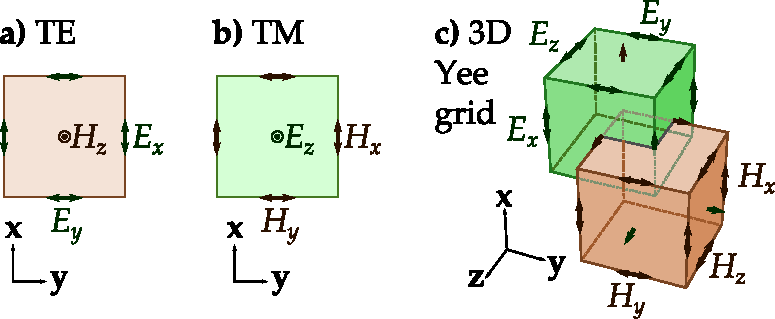
\includegraphics[width=12cm]{img/FDTD_Yee_grid_2d-3d.pdf}
\end{figure}

The error due to the numerical dispersion is in most FDTD implementations reduced from first to second order ($\propto \Delta x^{-2}$ with regards to the voxel size $\Delta x$) by using a \textit{staggered grid}, which, in three dimensions, is also known as Yee grid \cite{yee1966numerical}. All six field components are expressed in different points within the voxel, as is illustrated in Fig. \ref{fg_fdtd_yee}c with the upper left (green) cube denoting the elementary one. 
%This is similar to the advantage of trapezoid integration instead of direct summation. % TODO figure
Likewise, the update of electric and magnetic fields have to be interlaced also in time (as a so-called \textit{leapfrog} process). When accessing the field values at a given position and time, each field component has to be properly averaged between nearest points in the grid, and between nearest update times.
% NOTE FK: This can lead to errors especially at the boundaries with vacuum.

By adequate averaging of permittivity on the boundaries of materials, this error can likewise be reduced to the quadratic order with regards to $\Delta x$. Various averaging approaches have been studied in the literature \cite{oskooi2010meep}. Arithmetic averaging of permittivity with a weight proportional to the voxel volume occupied by the material is perhaps the most intuitive one, but it often gives wrong results, and  sometimes it is even worse than no averaging at all \cite{farjadpour2006improving,deinega2007subpixel}. 

In case of a single planar interface between two different materials under general orientation, the arithmetic average of the permittivities $\varepsilon_r$ is correct only for the electric field component \textit{parallel} with the interface, whereas the component \textit{perpendicular} to the interface requires to apply this weighted averaging to the reciprocal value of permittivity, $\varepsilon_r^{-1}$, instead. Such an approach is extremely accurate for all interfaces with low curvature, but it requires the FDTD simulation to define the permittivity as a $3\times 3$ tensor array (even in the simple case of isotropic materials being used). 

The situation gets even more  complicated if the materials have dispersive permittivity, where also the weighting coefficients of both media need to be frequency-dependent, and another sophisticated approach has to be employed \cite{deinega2007subpixel,hamm2013dispersive}. Such a level of elaboration easily leads to computation requirements that may outweight the benefit of averaging, and accordingly no averaging was used for the simulations presented in this thesis. 

In general, the effect of discretization in FDTD simulations can be easily identified by comparing results from two simulations that only differ by the grid resolution. It is a good practice to verify that such an error is negligible whenever a new simulation is tested.
%}}}
\paragraph{Temporal discretisation} %{{{
While the spatial resolution $\Delta x$ can be relatively freely set depending on the accuracy expected by the user, the \textit{temporal resolution} $\Delta t$ is related to $\Delta x$ by rules that will be discussed below. Generally, if $\Delta t$ is set too high, the simulation will get numerically unstable, yielding unrealistic or even infinite values.  %  slowing down the computation and

In the literature, one often encounters that the \textit{Courant factor} $S$ is used instead of the description in terms of $\Delta t$,
\begin{equation} S~= \frac{c \Delta t}{\Delta x}, \label{eq_courant}\end{equation}
In words, the Courant factor $S$ denotes what part of a FDTD cell the light can travel within one time step. 
The reason for introducing this quantity consists in the Maxwell equations [Eq. (\ref{eq_me1}-\ref{eq_me4})] being scale invariant, which holds also for the field update routine in FDTD when materials with frequency-independent permittivity are used. Therefore, when the resolution $\Delta x$ is changed, $S$ can be a well-chosen built-in constant and the time resolution given by Eq. (\ref{eq_courant}) ensures that the simulation does not go unstable.

FDTD obviously ceases to be scale-invariant whenever the properties of the materials depend on the frequency, which is needed for many realistic simulations. Then it appears more convenient to the autor to formally introduce yet another quantity, a \textit{critical frequency} $f_c$:
\begin{equation} f_c := \frac{1}{\pi \, \Delta t} \equiv \frac{c}{\pi\, S\, \Delta x} \label{eq_fc}\end{equation}
Note that this frequency is different %(i.e. $\pi$-times lower) 
than the frequency of time-stepping cycles is. It is however the value of $f_c$, and its relation to the model of materials used, that are of key importance for assessing the numerical stability of simulation. %% TODO-FK: cite

%A fundamental rule is the way how materials are defined in FDTD.
%}}}
\paragraph{Definition of materials for the FDTD method} %{{{
\label{def_of_mat}

\begin{figure}[t] \caption{Plots of complex permittivity ${\epsrl}_o(\omega)$ of titanium dioxide (rutile), for an ordinary ray. The above plot has a linear vertical scale, while the bottom plot displays the same quantity using the scale that is $-\log(-\varepsilon_r)$ for $\varepsilon_r<-1$; linear for $-10<\varepsilon_r<10$ and $\log(\varepsilon_r)$ for $\varepsilon_r > 1$. The second approach is more suitable for plotting permittivity in the following discussion.} \label{fg_tio2eps} \centering 
	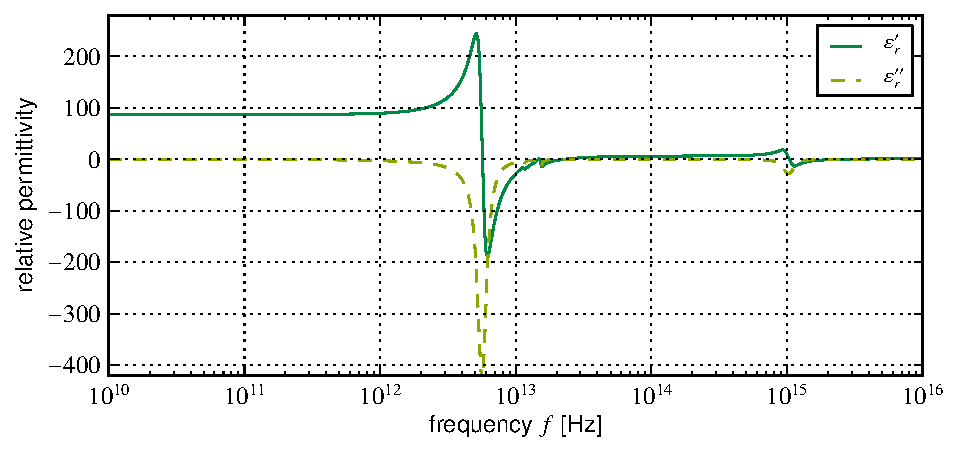
\includegraphics[width=14cm]{img/epsilon_TiO2_linear.pdf}
	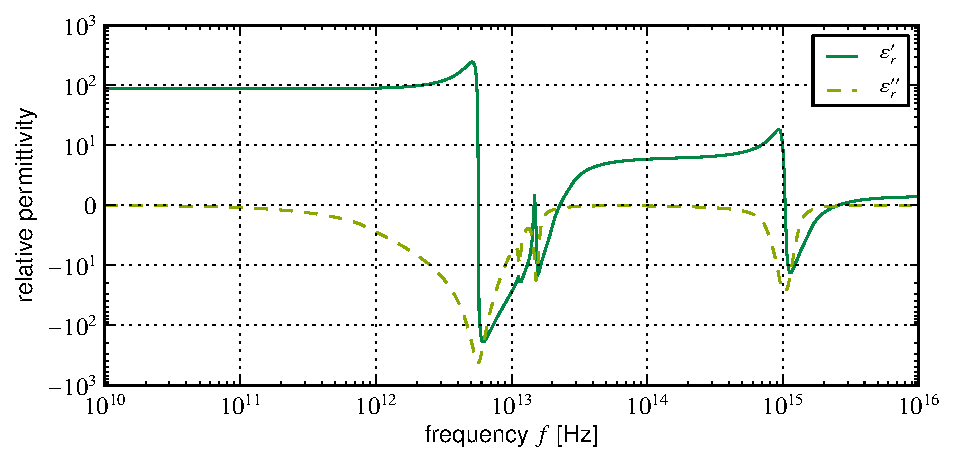
\includegraphics[width=14cm]{img/epsilon_TiO2_symlog.pdf}
\end{figure}


As described in Chapter \ref{chap_lorentzmedia}, Eqs. (\ref{eq_lorentz_eps}, \ref{eq_lorentz_mu}), the (local) response of usual media to an electromagnetic wave can be well approximated by a set of Lorentz oscillators, each of which is defined by three positive real numbers: its resonance angular frequency $\omega_{0}$, damping rate $\gamma$ and oscillator strength $F$. % todo cite 

%It is not possible to directly supply the permittivity as an arbitrary function of frequency from fundamental reasons. 
%We thus return to the local Drude-Lorentz theory, with a due emphasis on the definition of materials in FDTD.
% we focus on this topic because in literature, either general theory is discussed, or just single working model  is used. We try to develop reliable rules for employing the FDTD to simulate realistic structures under as general circumstances as possible.
FDTD, being a time-domain method, uses %% TODO-FK why?
a computationally efficient description of the media in a similar  form, with the difference that the nondispersive part of relative permittivity $\varepsilon_{r\infty}$ can be chosen as a real number. 
\begin{equation} \epsrl(\omega) = \varepsilon_{r\infty} + \sum_{m=1}^M \frac{F_m}{\omega_{0m}^2 - \omega^2 + \ii\omega\gamma_m} \label{eq_lorentz_eps_fdtd} \end{equation}
An illustration of a complex permittivity spectrum for titanium dioxide in its rutile allotrope is shown in Fig. \ref{fg_tio2eps}. As its crystal is birefringent, only one permittivity component, denoted as the \textit{ordinary}, from the tensor in Eq. (\ref{eq_epstensor}) was selected. 


% TODO add a spectrum + table for SiO2?
%			or exp(-i omega t)					-> FFT has to be conjugated (??)


%A rough list of the most important phenomena follows. 
%\begin{table}[ht]   \caption{}  \label{tb_phenomena} \centering 
%\begin{tabular}{lcr}
 %\toprule
%Frequency $\omega_0/(2\pi)$         & Contribution $\Delta\varepsilon_r$ & Physical phenomenon	\\
 %\hline
%---									& 0--10000 &	& Rotation of polar molecules	\\
%1 THz -- 30 THz						& & Vibration of atomic lattice	\\
%200 THz - 1000 THz					& &	\\
 %\bottomrule
 %\end{tabular} \end{table}
%\begin{enumerate}
 %\item{In the low frequency and microwave range (up to 1 THz), rotation and reorganisation of polar molecules plays the major role in the medium polarizability. } 
 %\item{Depending on the hardness and density of the medium, the lattice vibrates at frequencies between 1 and 30 THz.} 
 %\item{The frequencies corresponding to  electron motions of solids are in near-infrared, optical or ultraviolet ranges (roughly 200-1000 THz).}
 %\end{enumerate}
%If the medium is conductive, 



%}}}
\paragraph{Conditions of stability in FDTD}%{{{
%it was noted above that too high frequency of oscillators may introduce instability. 
%An important parameter is the critical frequency of the simulation, $f_c$ defined as 
% \begin{equation} f_c = \frac{c}{\pi \, C \, \Delta x},\label{eq_}\end{equation}
% where the \textit{Courant factor} $C$ is usually set to $C:=0.5$ and $c \approx 2.998 \cdot 10^8$ m/s is the speed of light. The voxel size thus determines the critical frequency; in a simulation typical for this thesis, $\Delta x := 2$ $\upmu$m and the critical frequency $f_c \approx 95$ THz lies in the mid-infrared. For simulations in visible range with $\Delta x := 50$ nm, and $f_c \approx 3800$ THz, that is, in the regime of hard UV radiation.

%The critical frequency may be viewed as the upper limit where an FDTD simulation gives plausible data. 

% TODO write that this holds only for a nonmagnetic medium
The author observed that $f_c$ determines the constraints for the simulation stability simultaneously in two ways:
\begin{enumerate}
 \item{The resonance frequencies must be lower than the the critical frequency,  %% TODO get a proof, or some citation, or cite MEEP sources where S.G.Johnson wrote a routine about this
\begin{equation} \frac{\omega_{0m}}{2\pi} < f_c, \text{ for all oscillators, } % \forall m \in \{1,2 \ldots M\}, \label{eq_fdtd_stability}
\end{equation}
independent of what the strength $F_m$ or damping rate $\gamma_m$ of the oscillator is. 
%This relates to the above note about expressing all high-frequency oscillators in the form of the high-frequency (static) permittivity. . 
} 
 \item{For all frequencies higher than the critical frequency $f_c$, the real part of the permittivity, as given by Eq. (\ref{eq_lorentz_eps_fdtd}), must exceed a minimum value given by the Courant factor $S$,
\begin{equation} \varepsilon_r'(2\pi\,f) > 3 S^{2} \equiv 3 \left( \frac{c \Delta t}{\Delta x} \right)^{2} \text{ for } \forall f \geq f_c. \label{eq_fdtd_stability_realp}\end{equation}  } % TODO verify whether the limit is eps>0 or e.g. eps>0.5 or whatever 
A geometrical interpretation of this rule is that an instability is introduced when any wave with a frequency above $f_c$, can travel more than $1/\sqrt{3}$ of one FDTD cell size within one time step. 
Note that in a nonmagnetic medium, the traveled distance is $$\frac{c\Delta t}{\sqrt{\varepsilon_r'}}.$$
\end{enumerate}
The FDTD simulation will become unstable if any of these rules is broken. The error from the instability initially arises from an inevitable numerical noise at the boundary of the problematic material and grows exponentially. It can be identified as a pixel-wise checkerboard pattern on the field snapshot. Later, the field visualisation usually returns black images as the numerical infinity is reached within several tens of FDTD steps. 

\paragraph{Choice of the Courant factor}%{{{
Provided that a part of the simulation volume is empty vacuum ($\varepsilon_r'=1$), Eq. (\ref{eq_fdtd_stability_realp}) clearly determines the \textit{maximum value of Courant factor} 
$$S_{max} = 3^{-1/2}\approx0.577.$$
In practice, a slightly more conservative choice is made that provides a safe margin for the numerical imprecision: 
\begin{equation} S:= 0.500 \quad \rightarrow \quad \varepsilon_r'(2\pi\,f)> 0.75, \quad \forall f \geq f_c. \label{eq_courant_choice}\end{equation}
For any material with a problematic high-frequency permittivity, $\varepsilon_r'(2\pi\,f_c) \in (0, 1)$, some low value of $S$ can be found that makes the simulation stable against the latter rule. Simultaneously, the critical frequency shifts up, so potential problems with the first rule may be alleviated, too. This is done, however, at the price of scaling up the number of required FDTD steps, so usually a reasonable change of the material definition is made instead of reducing $S$.
%% TODO note that the same would apply to permeability mu, but it usually does not have problematic oscillator parameters

%%% TODO 
%%% This is related to the \textit{Courant criterion} \cite{taflove2005book} that states for a nondispersive medium of permittivity $\varepsilon_r$ that 
%%% $$\Delta t = S\,\frac{\Delta x}{c}  <  \frac{\sqrt{\varepsilon_r}}{\sqrt{3}}   \frac{\Delta x}{c}$$, as $S < n_{min}/\sqrt{\text{dim}}$ % TODO
%%% i.e.
%%% $$c \Delta t / n_{min} < \Delta x / \sqrt{\text{dim}} $$
%%% which can be reformulated that   %TODO TODO

%  /* Return true if the discretized Lorentzian ODE is intrinsically unstable,
%     i.e. if it corresponds to a filter with a pole z~outside the unit circle.
%     Note that the pole satisfies the quadratic equation:
%  			(z + 1/z - 2)/dt^2 + g*(z - 1/z)/(2*dt) + w^2 = 0
%     where w = 2*pi*omega_0 and g = 2*pi*gamma.   It is just a little
%     algebra from this to get the condition for a root with |z| > 1. */
%  static bool lorentzian_unstable(double omega_0, double gamma, double dt) {
%    double w = 2*pi*omega_0, g = 2*pi*gamma;
%    double g2 = g*dt/2, w2 = (w*dt)*(w*dt);
%    double b = (1 - w2/2) / (1 + g2), c = (1 - g2) / (1 + g2);
%    return b*b > c && 2*b*b - c + 2*fabs(b)*sqrt(b*b - c) > 1;
%  }
%}}}


%The first rule of $\omega_0/2\pi < f_c$ was observed to be very strict
%}}}
\paragraph{Practical aspects of material definition} %{{{
In all realistic media, the frequencies of different oscillators span over many orders of magnitude, and an accurate medium model would need to determine excessively big number of oscillators. Not all oscillators should be accounted for in a given FDTD simulation, however. 

\begin{figure}[t] \caption{Permittivity plot for titanium dioxide, similar to Fig. \ref{fg_tio2eps}. 
%Compared to the exact model of permittivity (green line), the model with reduced number of Lorentz oscillators was plotted (black line). 
The region forbidden by the stability rules is yellow shaded (above $f_c = 95$ THz and below $\varepsilon_r < 0.75$). The exact model for TiO$_{2}$ (green line) would be definitely unstable due to violating both stability conditions. The numerically stable model for the frequency range of interest up to ca. 10 THz (black line) has all high-frequency oscillators substituted by an increased value of $\varepsilon_{r\infty}$. Solid and dashed lines denote the real and imaginary parts, respectively. } \label{fg_tio2eps_stripped} \centering 
	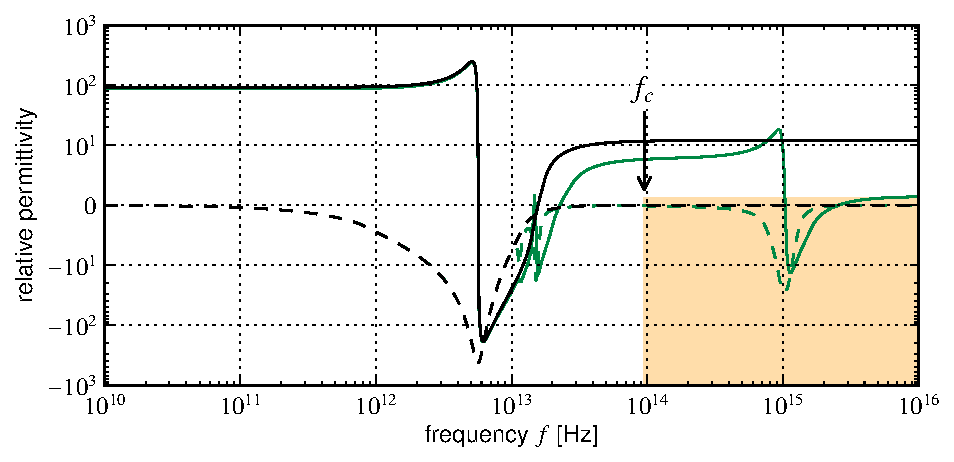
\includegraphics[width=14cm]{img/epsilon_TiO2stripped_symlog.pdf}
% full:
      % self.eps = 1
      % self.pol = [
      %         {'omega':5.67e12, 'gamma':1.05e12, 'sigma':50+90*extraordinary},      
      %         {'omega':11.43e12, 'gamma':.495e12, 'sigma':0.9*extraordinary},            
      %         {'omega':15.24e12, 'gamma':.72e12, 'sigma':2.6*extraordinary},            
      %         {'omega':1.0e15, 'gamma':.15e15, 'sigma':2.8 + .5*extraordinary},     ## imprecise two-Lorentzian approximation in UV
      %         {'omega':1.08e15, 'gamma':.15e15, 'sigma':2 + .4*extraordinary}            
% reduced: self.eps = 12.  self.pol = [ {'omega':5.67e12, 'gamma':1.05e12, 'sigma':50+30.} ]
\end{figure}

First of all, high-frequency oscillators would make the simulation unstable.
Aside from this, adding overly many oscillators is also inefficient, because each oscillator defined increases the computing difficulty in FDTD. 
It is therefore advisable to keep the oscillator number to an acceptable necessary minimum, and to describe the material within some frequency range of interest (FRoI) % TODO  define range of interest
only:
\begin{enumerate}
 \item{
%Often the first step in processing FDTD results lies in converting them to frequency domain via Fourier transform. 
The upper bound of the FRoI is limited by the numerical stability as stated above. Mostly, a more strict limit is imposed by the spatial resolution of the simulation: in a high-permittivity material, too high frequencies correspond to wavelengths similar to the voxel size (or even smaller than it), leading to a significant inaccuracy. 

Each oscillator far above the frequency of interest shall be expressed only as a constant added to the nondispersive part of permittivity $\varepsilon_{r\infty}$. The contribution of an $m-$th oscillator is given by Eq. (\ref{eq_delta_eps}) as 
$$(\Delta \varepsilon_r)_m = \frac{F_m}{\omega_{0m}^2}.$$ 
If some of the high-frequency oscillators introduces significant dispersion or losses in the FRoI, it it should not be eliminated this way. This usually concerns the oscillator that is the closest above FRoI, and it usually can be kept without causing instability.
} 
 \item{
Very low frequencies, corresponding to wavelengths much greater than the whole simulation volume, are theoretically accessible with a long-enough FDTD simulation, but the FRoI usually does not reach zero frequency, mostly for practical reasons. If needed, the low-frequency phenomena can often be computed more efficiently in a separate simulation with a lower resolution or even with different numerical methods.

The oscillators at too low frequencies can therefore be omitted without any change to the behaviour within the FRoI. One important exception is the low-frequency oscillator that defines the conductive behaviour, as described below.
} 
 \end{enumerate}
%}}}
\paragraph{Drude model for conductive media} \label{chap_fdtd_drude}  %{{{
The Drude model assumes a zero resonance frequency, i.e., the relative permittivity in the form
\begin{equation} \epsr(\omega) = 1 + \frac{\omega_p^{2}}{0 - \omega^{2} + \ii\gamma\omega} = 1 - \frac{\omega_p^{2}}{\omega^{2} - \ii\gamma\omega}, \label{eq_drude_eps}\end{equation}
where $\omega_p$ and $\gamma$ are two independent parameters that describe the metal: 
\begin{itemize}
 \item{$\omega_p$ is the \textit{plasma frequency}, at which the real part of permittivity crosses zero. The physical consequence is that for $\omega > \omega_p$ the medium allows the transverse electromagnetic wave to propagate through. 
%The angular frequency of $\omega_p$, the longitudinal (electric) waves oscillate. 
%The quasiparticle associated with the oscillation of the charge in bulk conductive medium, a \textit{plasmon}, has given the name to $\omega_p$. % TODO add a relation to the chapter on "dispersion in local media"
 } 
 \item{$\gamma$ can be understood as the \textit{rate of exponential decay} of the medium response to an impulse, similar as in the Lorentz model. The Drude model was conceived in the early 20th century, with the simplified hypothesis that electrons would be freely propagating particles that undergo 
	% mutual elastic %% +FK?
collisions 
	with the atoms %% -FD?
at an average frequency $\gamma$. Upon the colision, their 
	%speed would either drop to zero, or (equivalently) %% -FD?
	velocity vector % + FK
would be randomized. 
%Although the mechanism of resistivity is more complicated than this,  -FD
The Drude model often provides a very good approximation of the metallic-like response.
The parameter $\gamma$ is commonly denoted as the \textit{scattering frequency}.} 
 \end{itemize}
%Both have the dimension of $\mathrm{rad\; s^{-1}}$. 
The Drude model can thus be considered a specific case of a Lorentz oscillator with $\omega_0 = 0$, and oscillator strength given by $F = \omega_p^2$. 
Obviously, using Eq. (\ref{eq_delta_eps}) to compute the contribution of the Drude term to the real part of permittivity would give infinite values, as static electric field can displace unlimited amount of charge in a conductor.

If $\gamma$ is nonzero, the permittivity is a complex function and it can be separated into its real and imaginary part $\varepsilon_r = \varepsilon_r'+\ii\varepsilon_r''$ by expanding the fraction in (\ref{eq_drude_eps}) by complex conjugate of its denominator
\begin{equation} \varepsilon_r = 1 - \omega_p^{2} \cdot \frac{\omega^{2} + \ii \gamma \omega}{\omega^{4} + \gamma^{2} \omega^{2}} = 
		\underbrace{\left(1 - \frac{\omega_p^2}{\omega^2+\gamma^2}\right) }_{\text{real part } \varepsilon_r'}
+ \ii	\underbrace{\left(\frac{-\omega_p^2\gamma}{\omega^3 + \gamma^2\omega}\right) }_{\text{imaginary part } \varepsilon_r''}.
\label{eq_drude_eps_loss}\end{equation}
%The real part $\varepsilon_r'$ indicates capacitive or reactive behaviour of the metal. The imaginary part $\varepsilon_r''$ describes losses which may arise either from 
% \underbrace{ }_{\text{}}
The low- and high-frequency limits of permittivity given by the Drude model are:
\begin{equation} \lim_{\omega \to 0} \varepsilon_r' = 1-\frac{\omega_p^2}{\gamma^2}, \quad \quad  
				 \lim_{\omega \to 0} (\varepsilon_r'' \cdot \omega) = -\frac{\omega_p^2}{\gamma},\label{eq_drude_limlow}\end{equation}
\begin{equation} \lim_{\omega \to +\infty} \varepsilon_r' = 1, \quad \quad  
				 \lim_{\omega \to +\infty} (\varepsilon_r'' \cdot \omega^3) = -\omega_p^2 \gamma. \label{eq_drude_limup}\end{equation}
We can see that in the low-frequency limit, the imaginary part of permittivity diverges (while its real part has a finite value). In the high-frequency limit, the metal permittivity approaches that of vacuum, i.e. $1+0\ii$.
%}}}
\paragraph{Low- and high-frequency limits of conductivity in the Drude model}%{{{
The notion of \textit{conductivity} is widely used to describe metals and doped semiconductors, i.e. media where the response to the electric field is characteristic by the motion of free charge carriers. 
Generally, both permittivity $\varepsilon_r(\omega)$ and conductivity $\sigma(\omega)$ are complex functions of the angular frequency $\omega$. As long as the approximation of a negligible spatial dispersion is used, each of them is fully determined by the other function. % maybe even if spatial dispersion is nonzero -> check this?
For clarity, we avoid using the conductivity in the rest of the thesis except this chapter.

The relation between $\varepsilon_r(\omega)$ and $\sigma(\omega)$
 can be derived by realizing that the current in a material is always caused by movement of charges with a density $\rho$ and average velocity $\mathbf{v}(t)$. The conduction and polarisation currents are not distinguished here, as their density is given as $\rho \mathbf{v}(t)$ in both cases. When current is excited by a harmonic electric field $E(t) = \mathrm{e}^{\ii\omega t}$: %TODO FIXME explain rho.n, use i omega t instead of -i omega t, check again...
\begin{equation} \rho \mathbf{v}(t) = \sigma(\omega) E(t) = \sigma(\omega) \mathrm{e}^{\ii\omega t}, \quad\text{ (conduction approach -- Ohm law)} \label{eq_rho_n1}\end{equation}
\begin{equation} \rho \mathbf{v}(t) = \varepsilon_0 \varepsilon_r(\omega) \frac{\partial E(t)}{\partial t} = \ii \omega \varepsilon_0 \varepsilon_r(\omega) \mathrm{e}^{\ii\omega t} . \quad\text{ (displacement current approach)} \label{eq_rho_n2}\end{equation}
Both above equations describe the same quantity, so
\begin{equation} \sigma(\omega) = \ii \omega \varepsilon_0 \varepsilon_r(\omega), \quad  \text{and} \quad  \varepsilon_r(\omega)  = \frac{\sigma(\omega)}{\ii \omega \varepsilon_0}. \label{eq_drude_sigma}\end{equation}
Thus, a dielectric medium with a real constant permittivity has \textit{imaginary} conductivity, the magnitude of which grows with frequency (cf. the admittance of a capacitor). A conductor with a real constant conductivity has complex permittivity, whose imaginary part diverges in the low-frequency limit. 
% NOTE: eps_r = eps_r' + i eps_r'',   
% sigma = sigma' + i sigma'' == i omega eps0 eps_r == i omega eps0 eps_r' - omega eps0 eps_r''
% therefore a material can be described also using real epsilon = eps_r', and real conductivity sigma' = -omega eps0 eps_r''

\begin{figure}[t] \caption{Permittivity and conductivity plot for gold; the yellow region, forbidden by the stability rules, is the same as in Fig. \ref{fg_tio2eps_stripped}. The exact model of gold \cite{rakic1998optical} 
(red) is compared to the lossy Drude model with Lorentz oscillators substituted by $\varepsilon_r$ (blue), and for illustration, also to the lossless Drude model with scattering frequency set to zero (grey). Obviously, none of these models is numerically stable if $f_c = 95$ THz.
\\The bottom plot shows the conductivity of these three models as given by Eq. (\ref{eq_drude_sigma}).}
\label{fg_Au_models} \centering 
	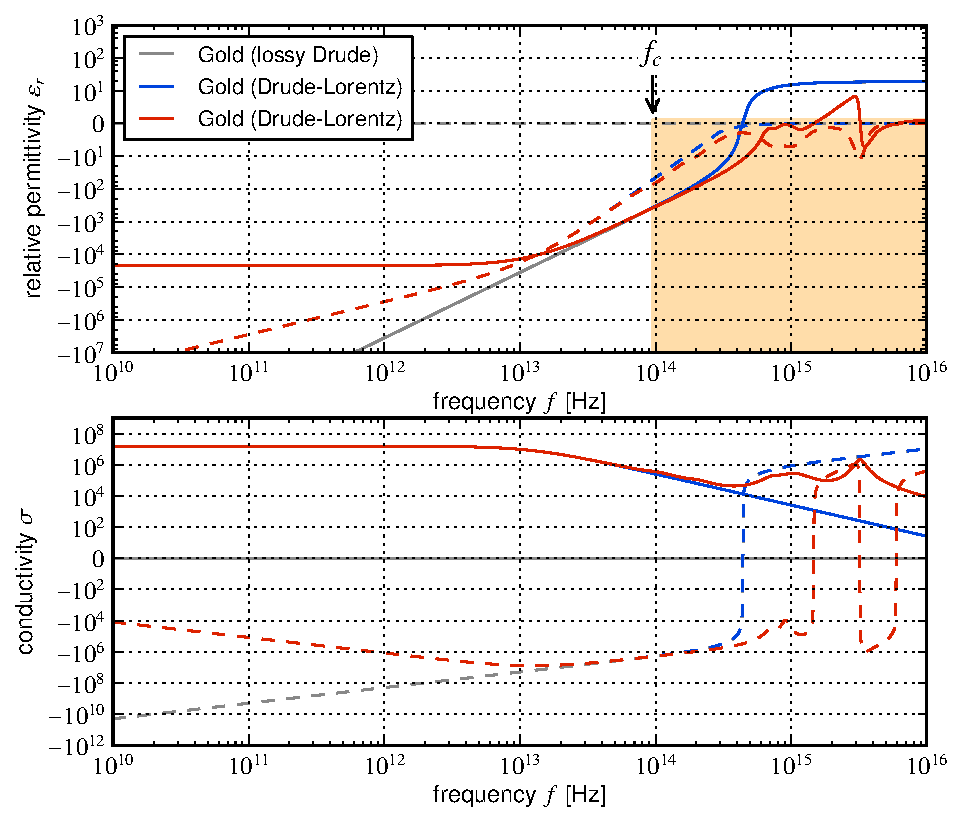
\includegraphics[width=14cm]{img/epsilon_Au_models_llgrey.pdf} % Scattering freq of gold = 12.8 THz
\end{figure}


Using the above relation (\ref{eq_drude_sigma}) to convert the metal permittivity $\varepsilon_r(\omega)$ into conductivity $\sigma(\omega)$, and substituting the Drude-model permittivity (\ref{eq_drude_eps_loss}), we obtain
\begin{equation} \sigma(\omega) = \ii \omega \varepsilon_0 \varepsilon_r(\omega)= \ii\omega \varepsilon_0 \varepsilon_r'(\omega)  -  \omega \varepsilon_0 \varepsilon_r''(\omega) = 
	\ii \underbrace{\varepsilon_0 \left(\omega - \frac{\omega_p^2\omega}{\omega^2+\gamma^2}\right)}_{\text{imaginary part } \sigma''}  + 
		\underbrace{\varepsilon_0\frac{\omega_p^2\gamma}{\omega^2+\gamma^2}}_{\text{real part } \sigma'}. \label{eq_drude_sigmaeps1}\end{equation}
We may now express the low- and high-frequency limits also for conductivity:
\begin{equation} \sigma_{LF} := \lim_{\omega \to 0} \sigma' = \frac{\omega_p^2\varepsilon_0}{\gamma}, \quad \quad  
				 \lim_{\omega \to 0} (\sigma'' / \omega) = \varepsilon_0 - \frac{\omega_p^2 \varepsilon_0}{\gamma^2} , \label{eq_drude_sigmalimlow}\end{equation}
\begin{equation} \lim_{\omega \to +\infty} (\sigma' \cdot \omega^2) = \varepsilon_0\omega_p^2\gamma, \quad \quad  
				 \lim_{\omega \to +\infty} (\sigma'' / \omega) = \varepsilon_0. \label{eq_drude_sigma_limup}\end{equation}
Let us note again that in the literature that uses the negative phase convention $e^{-\ii \omega t}$, the resulting $\varepsilon_r(\omega)$ and $\sigma(\omega)$ are complex conjugated to the results above. 
%}}}
\paragraph{Defining resistive metals for stable low-resolution simulations} %{{{
Simulations in the optical range are relatively safe in terms of numerical stability. From Eq. (\ref{eq_fc}) it follows that the resolution of $\Delta x = 50$ nm, suitable for the NIR/visible spectrum, yields a critical frequency of $f_c = 3.82\cdot 10^{15}$ Hz ($\lambda = c/f_c \approx 78$ nm), which is far above the plasma frequency of metals or other conductors. Accordingly, no changes to the Drude model are usually needed to be made, although the simulation may run faster if one or more Lorentz terms outside FRoI can be omitted.
%If high precision of the metal model is needed, one is also free to add one or more Lorentz oscillators in the optical/UV range to refine the shape of permittivity.
 
Realistic simulations of metals at lower resolutions however require taking measures to ensure stability, as the critical frequency $f_c$ is reduced below the plasma frequency of most metals when $\Delta x \gtrsim 200$ nm. % TODO check this
A trivial approach is to drastically reduce the Courant factor $S$ so that $f_c$ remains above plasma frequency. Although this should reliably avoid the instability, it would be so at the expense of scaling the computational time. As a general rule, lower resolution is typically chosen for larger structures, where also all investigated processes accordingly happen on a longer timescale.
%Drude model is known to introduce negative permittivity up to optical range, so 
%Assuming the critical frequency is far below the optical range, the Lorentz oscillators can be certainly neglected. Nonetheless, negative permittivity above critical frequency still introduces instability, which has to be resolved. 

For simulations with lower resolution, it is much more efficient to replace the exact Drude model with its approximation that maintains the same low-frequency limit of conductivity $\sigma_{LF}$, but has positive permittivity around the critical frequency and above it. 
This formally inverts the relations that describe the material:
\begin{itemize}
\item{
For \textit{high-resolution simulations}, $\omega_p$ and $\gamma$ are given as experimental properties of the metal, which determine the lower limit $\sigma_{LF} = \omega_p^2\varepsilon_0\gamma^{-1}$ and the nondispersive part of permittivity $\varepsilon_{r\infty} = 1$ is fixed to that of vacuum. 
} 
\item{
For \textit{low-resolution simulations}, the situation is the opposite: $\sigma_{LF}$ is given as an experimental property, $\gamma < 2\pi f_c$ is given by the critical frequency, % TODO describe why so
whereas $\varepsilon_{r\infty}$ and $\omega_p$ are to be determined from the previous two input parameters.
} 
\end{itemize}

%%% TODO
%%% 	% In this section we develop the strategy to determine the correct combinations of  $\gamma < 2\pi f_c$, $\varepsilon_{r\infty}$ and $\omega_p$.
%%% 	% The value of $\gamma$ is also limited to be lower than $2\pi f_c$, so its value is fixed to be as close to $2\pi f_c$ as possible. % TODO ...is it? verify and add to the rules for stability written above
%%% 	 The values of the plasma frequency $\omega_p$ as well as the  $\varepsilon_{r\infty}$ remain to be freely manipulated.
%%% 
%%%     $$ \gamma = 2\pi f_c \cdot gammafactor $$
%%%     % test when unstable -> reduce self.gamma by 100 -> test again -> finally write automatic selection of value
%%% 
%%%     % Knowing the scattering frequency gamma, the virtual plasma frequency is now determined by lfconductivity
%%%     $$ \omega_p = \sqrt{\frac{\gamma \sigma_{LF}}{\varepsilon_0}} $$
%%% 
%%%     % The following step is required for FDTD stability: 
%%%     % Add such an high-frequency-epsilon value that shifts the permittivity to be positive at f_c
%%%     % If self.eps>1, the frequency where permittivity goes positive will generally be less than f_p
%%%     $$\varepsilon_{r\infty} = (\omega_p/(2\pi f_c))^2 \text{ or 1 if it would be lower} $$

%}}}
%\paragraph{Conductive media in FDTD} %{{{
%The resonance frequency $\omega_0$ is inversely proportional to the square root of the restoring force in the harmonic oscillator. A conductive medium is characteristic by having part of the charges that do not experience any restoring force, so they can be modelled by an oscillator with a resonance frequency approaching zero: $\omega_0 \rightarrow 0$; in practice any value lower than the inverse of simulation time gives expected results.
%When $\omega_0$ is reduced to small values, the oscillator epsilon difference $\Sigma = \Delta \varepsilon_r$ has to be upscaled accordingly to keep the plasma frequency constant.
%When $\omega_0$ is reduced to small values, the oscillator strength $F$ shall be kept constant?
%}}}
\paragraph{Debye media in FDTD} \label{fdtd_debye} %{{{
The Lorentz model can be employed also to define overdamped oscillators, corresponding to the processes where  $\gamma \gg \omega_0$, i.e. the inertia is negligible.
A typical example is the  reorientation of polar molecules in liquids or solids. 

It can be shown that for $\gamma \gg \omega_0$, the peak in $\varepsilon_r''(\omega)$ lies approximately on the frequency $\omega_p^{2}/\gamma$. The spectral width of such a peak is proportional to its central frequency. 
% TODO figure illustrating this

\begin{table}[ht]   \caption{Comparison of Lorentzian types and corresponding physical phenomena}  \label{tb_lorentzians} \centering 
\begin{tabular}{cc|cc}
 \toprule
\textbf{Charges are}	& \textbf{Inertia is}				& \textbf{Phenomenon}				& \textbf{Example}		 \\
 \hline
Bound		& Significant				& Lorentz oscillator					& \shortstack{optical phonons, \\electronic levels,\\ molecular vibration \\or rotation in gases}	\\
 \hline
Bound		& Negligible				& Debye relaxation						& \shortstack{molecular rotation \\in solids or liquids} \\
 \hline
Free unbounded	& Significant				& \shortstack{Reactive\\(plasmonic) medium}			& \shortstack{colisionless plasma, \\metals (from mid-infrared\\to optical range)} \\
 \hline
Free unbounded	& Negligible				& Resistive medium						& \shortstack{doped semiconductors,\\\newline metals (in far-infrared\\ range and below)} \\
 \bottomrule
 \end{tabular} \end{table}
%}}}
% TODO? \paragraph{Selection of FDTD implementations} %{{{
% note about the meep peculiarity of notation: 'omega'=omega0/2pi , 'gamma'=gamma/2pi, 'sigma'=Deltaeps = F/omega0^2
%MEEP, OpenEMS, B-Calm, gSvit, EMTL, ..
%}}}

\subsection{Finite-difference frequency-domain method} % TODO
\paragraph{Principle} 
When the procedure for one time-step in FDTD is defined, it can serve as the linear operator $\mathcal L$ in the generic formulation of the eigenfunction problem:
$$\mathcal{L} \psi = e^{\ii \omega t} \psi,$$
where the function $\psi$ represents either of the electric or magnetic fields. The particular form for the linear operator $\mathcal{L}$ is  
as has already been developed for the proof of the Bloch theorem in Eq. (\label{eq_eigen_e}).

Numerically, the problem can be expressed as a simultaneous optimization of the $\E, \HH$ fields shape such that one time-stepis identical to phase rotation of the field at the given angular frequency $\omega$.
We remind that unless stated otherwise, the simulations use complex numbers to represent all field components.
For the optimization to be as efficient as possible, the authors of the simulation used, namely MEEP , chose the stabilized biconjugate gradient \cite{oskooi2010meep}. More information on the frequency-domain solver is on the project's website. % todo cite ab-init

The modes obtained by frequency-domain simulation can have arbitrary phase; sometimes the real part of either electric or magnetic field can be nearly zero. In such a case, the imaginary part thereof always gives sufficient amplitude to be plot accurately.


%}}}
\paragraph{Comparison to the time-domain computation} 
To verify their reliability, the results of the frequency domain simulation with frequency scanned were compared against the results from the time-domain simulation. \todo{add results from freq-domain test}

%%% Cons: inefficient, convergence not guaranteed
%%% Pros: very convenient once time-domain simulation is prepared
%%% In the latest meep version (1.2.1), nondispersive $\varepsilon_r, \sigma$ must be
%%% provided. This is facilitated by meep utils.py.
%%% 
%%% No limitation is known for the permittivity value in frequency-domain; however too exotic values can prevent the solver from converging.
%%% 

\subsection{Plane-wave expansion method} % TODO
\paragraph{Principles of PWEM} %{{{
Another algorithm used is the plane-wave expansion method (PWEM). This method works in the frequency domain and, being based on the eigenmode problem, its use is similar to the frequency-domain finite-difference solver (FDFD) described above, though it is based on directly solving a linear algebraic problem in contrast with the somewhat inefficient optimisation used in FDFD.
PWEM consists in expressing the structure permittivity in the inverse space, using spatial Fourier transformation. For any given wavevector, an eigenvalue problem can be solved, with boundary conditions fully determined by the wavevector as sketched in Chapter \ref{tight-binding}. The resulting eigenvalues are the frequencies of different modes in the folded dispersion curves.  


For the given wavevector, PWEM also gives the shape of the fields for each mode. This approach turns out to be easier and more reliable than running the frequency-domain solver in FDTD selecting the approximate frequencies of the band edges, so we mostly used PWEM to get an insight into the field distribution. 
As a convenient implementation of PWEM, we used the freely available program \textit{MPB} \cite{johnson2001mpb}, implemented by the same group as MEEP.
% Todo comments on MPB
%}}}
%  \paragraph{Comparison of PWEM to FDTD} %{{{ WTF
%  While the time-domain methods are very general, allowing to compute both periodic and non-periodic structures with losses or nonlinearity, some tasks may be better solved by more specialized methods. An example is the \textit{plane-wave expansion method} (PWEM), which is superior for efficient search of dispersion curves in periodic structures, and for the mode shapes at the band edges.
%}}}

%% \subsection{Transfer-matrix method} % TODO??

%% \paragraph{Principles of TMM} %{{{
%% \add{
%% The \textit{transfer-matrix method} (TMM, or also \textit{Abelès formalism} %% ref Abeles1950: recherche sur la propagation des ondes electromagnetiques...
%% ) provides an analytically exact and notably simple computation of the transmission of one-dimensional, layered structures. It has been applied e.g. for the design of antireflective layers, dielectric mirrors, defect-mode filters etc. It shall be noted that extensions of TMM for two- or three-dimensional computation also exist \cite{pendry1992_transfer_matrix}, \cite[pp. 71--77]{nemec2006phd}, enabling to compute,  in frequency-domain, e.g. the reflection and transmission of structures discretized in a grid. For simplicity, we describe the one-dimensional method.
%% 
%% The method is on dividing the structure into a sequence of homogeneous layers. For each layer, a $2\times 2$ \textit{transfer} matrix is prepared that relates the $\mathbf E$ and $\mathbf H$ of the forward and backward propagating waves. If the $m$-th layer has a wave impedance $Z_m$, refractive index $N_m$ and thickness $d_m$, the transfer matrix $\mathbb M^{(m)}$ is given as
%% \begin{equation} \mathbb M^{(m)} := \left(\begin{array}{cc} \cos\delta & (i/\gamma)\sin\delta \\ i\gamma\sin\delta & \cos\delta \end{array}\right), \quad\text{ where }\gamma:=1/Z_m\text{ and }\delta := k~N_m d_m.\label{eq_tmm1}\end{equation}
%% Multiplication of such matrices gives the overall transfer matrix of the layered structure, 
%% \begin{equation} \mathbb M^{(tot)} \equiv \left(\begin{array}{cc} m_{11} & m_{12} \\ m_{21} & m_{22} \end{array}\right) = \ldots \cdot \mathbb M^{(2)} \cdot \mathbb M^{(1)}. \label{eq_tmm2}\end{equation}
%% The overall reflection $r^{(tot)}$ and transmission $t^{(tot)}$ are then 
%% \begin{equation} r^{(tot)} = \frac{m_{11} + m_{12} - m_{21} - m_{22}}{m_{11} + m_{12} + m_{21} + m_{22}}, \quad\quad t^{(tot)}= \frac{2}{m_{11} + m_{12} + m_{21} + m_{22}}, \label{eq_rt_tmm}\end{equation}
%% if perpendicular only incidence is assumed and if the surrounding medium consists of air.
%% 
%% The TMM is instrumental not only for its obvious simplicity, but also for providing mathematical interpretation of observed phenomena and allowing to define arbitrary properties of the layers (whereas both FDTD and PWEM restrict e.g. the constituent permittivity to be positive).
%% }
%% %}}}

\subsection{Summary of numerical methods used} %{{{
This section describes several fundamentally different numerical methods for electromagnetic simulations. 
\begin{enumerate}
\item{Finite-difference time-domain (FDTD) is a time-marching method that describes the structure on an uniform grid, allowing to compute very general electromagnetic problems. Usually a short-time, broadband pulse excitation is used, which allows to resolve a broad spectrum at once by Fourier transform. In the following chapter, two fundamentally different setups for FDTD are described that provide similar information on the metamaterial.} 
\item{The finite-difference frequency-domain (FDFD) method uses the same discretisation as FDTD, but instead of time-marching and Fourier transforming the result, it searches for the field eigenmode at one given frequency by means of numerical optimisation. It is useful e.g. for mode analysis in complicated structures.} 
\item{The plane-wave expansion method (PWEM) reformulates the problem of a wave propagating in a periodic structure by means of linear algebra. At a given wave vector, it allows to find eigenmodes and eigenfrequencies in the structure. This can be in turn employed to efficiently retrieve the dispersion curves.} 
\item{The transfer-matrix method (TMM) also allows to find dispersion curves and field distribution. Although it can be extended to two or three dimensions, its one-dimensional implementation is most popular. Thanks to its simplicity, it can even give an analytical insight into the behaviour of planar structures.} 
\end{enumerate}

%}}}
\paragraph{Overview of other numerical methods} %{{{
Other numerical methods are used, too. Finite-element methods (FEM) approximate the structure with a custom mesh of triangles or tetrahedra. The advantage consists in describing the structure smoothly with a relatively low number of elements of variable density; the downside is that the mesh introduces additional entropy and the computation on the element is significantly slower compared to straightforward arithmetics in FDTD. FEM is usually used as a frequency-domain solver, though time-domain computations are possible, too. The efficiency of the FEM mesh is superior to the FDTD/FDFD uniform grid particularly for structures with great differences between scale, that is, when important tiny structures are surrounded by large free space. This was however not the case of the structures studied in this thesis.
%% TODO Boundary-element methods, Fourier modal method, rigorous coupled-wave analysis (RCWA), ... 
%% discontinuous Galerkin method

%}}}

% \begin{verbatim}
% 										FDTD				FDFD				PWEM				TMM
% nonperiodic structures					yes					yes					no					yes
% dispersive and lossy media				yes					yes					no					yes
% nonlinear media							yes					no					no					no
% computation of dispersion curves		yes*				yes*				yes+				(yes)
% mode analysis							(yes)				yes					yes					yes
% \end{verbatim}

\section{Simulation setups for metamaterial homogenization} % TODO
% TODO theoretically shown in works [12,13,14,15] and experimentally confirmed in [16] this techniqueis not applicable when the sample material experiences the resonance
%		[12] C.R. Simovski, S.A. Tretyakov, Phys. Rev. B 75 (2007)195111
%		[13] C.R. Simovski, Metamaterials 1 (2007)62
%		[14] C.R. Simovski, Metamaterials 2 (2008)169
%		[15] C.R. Simovski, Optics and Spectroscopy 107 (2008)726
%		[16] Kh.Chalapat, K.Sarvala, J.Li, G.S.Paraoanu, IEEE Transactions on Microwave Theory and Techniques 57 (2009)2257
The general electromagnetic methods, such as FDTD, FDFD or FEM, can be employed to a wide variety of electromagnetic problems. Thanks to their versatility, different ways exist to retrieve effective parameters of metamaterials. We implemented two of them, and other approaches are mentioned at the end of this section.
\subsection{Scattering parameters method}
\label{chapter_sparam}
\paragraph{Principle} %{{{
The scattering parameter retrieval, also known as the \textit{s-parameter}, \textit{distributed impedance} or \textit{Nicolson-Ross-Weir} (NRW) method \cite{nicolson1970measurement, weir1974automatic}, has been used since 1970s to experimentally retrieve the index of refraction $N$ and wave impedance $Z$ of a homogeneous material sample, originally in the microwave range. It is based on the fact that, using Fresnel-Airy formulas, as shown in the Appendix \ref{app_fresnel},
one can easily compute the transmission $t$ and reflection $r$ from a slab of any material, provided its thickness $d$, index of refraction $N$ and wave impedance $Z$ are known.  If $r,t$ are known instead, the Fresnel-Airy formulas can be inverted to yield $N$ and $Z$ of the material the slab consists of. The actual computation is thus denoted also as \textit{Fresnel inversion}.

Mathematically, this can always be done (see Appendix \ref{app_fresnel_inv}), and this method yields some \textit{effective} parameters, $\Neff$ and $\Zeff$, even when the homogeneous sample is replaced with an inhomogeneous structure, such as a layer of a metamaterial. As a great advantage of this approach, there is no requirement to inspect the fields inside the tested structure, as the retrieval is based only on the amplitude and phase of $r(f)$ and $t(f)$ outside the material. Thanks to its ease to realize both experimentally and numerically, with FDTD or other algorithms \cite{terao2011},
it has become a popular way to retrieve the effective metamaterial parameters. 

The most often mentioned issue of this method is that the solutions have infinitely many branches, and it is necessary to establish which one should be chosen, and why. In this chapter we describe that this can, in fact, be solved relatively easily, and in the Section \ref{section_result} it is shown that the outcomes may be quite surprising.
Aside from yielding multiple branches, the physical interpretation of the data can get even more intricate when effective parameters are to be assigned to an inhomogeneous slab of a metamaterial. Due attention has to be paid to minimize the intrinsic imprecision of this method, as well as to establish the limits of its applicability. 
%}}}
\paragraph{Simulation setup} %{{{
\begin{figure}[ht] \centering \caption{The setup of the FDTD simulation for the scattering parameter method
% TODO REWRITE, and add the X-Y-Z arrows to the figure}
} 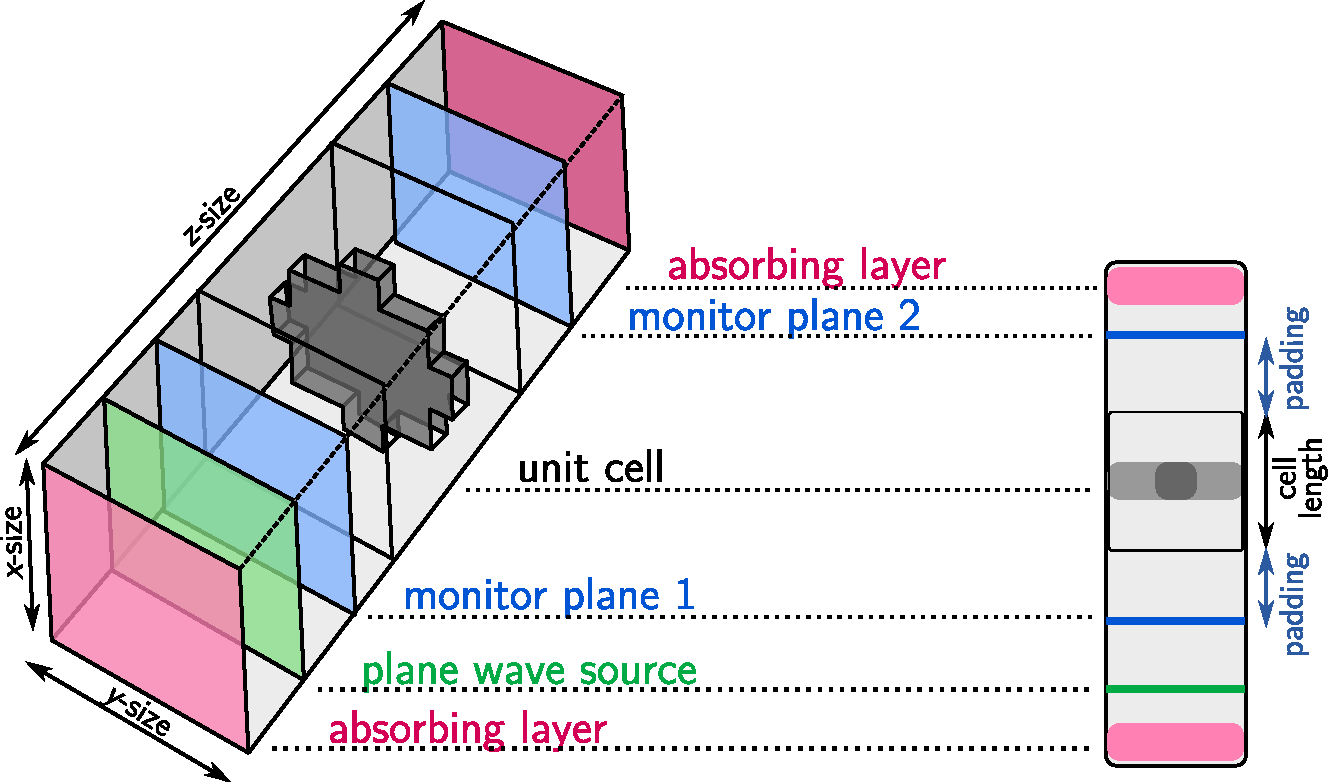
\includegraphics[width=12cm]{img/meep_geometry.pdf}  \label{fg_fdtd_sparam} \end{figure} %% 
The setup of the simulation is depicted in Fig. \ref{fg_fdtd_sparam}. The wave is emitted from the source plane (green rectangle) with a direction parallel to the $z$-axis. The temporal shape of the wave was not critical for the simulation; a very short pulse, with a spectrum spanning from the GHz range to ca. 5 THz was used. 

The periodic boundary conditions were set on the $x$- and $y$-axes, so that effectively an infinite metamaterial slab was simulated. On both faces perpendicular to the $z$ axis we added perfectly matched layers to absorb all radiation (pink blocks). The implementation used is based on gradually introducing imaginary part into the unit cell dimensions  to prevent reflections under arbitrary incidence angle, polarisation or frequency of the wave. There are different approaches for this problem \cite{oskooi2011distinguishing}. %, thus 

The electric and magnetic fields are averaged and recorded by the monitor planes (blue rectangles) in each simulation step.  

Passing through the first monitor plane, the wave enters the volume of the unit cell (delimited by empty rectangles) and interacts with the structure. A part of its energy is reflected back, a part passes through and part may be dissipated if the structure was lossy. The fields that passed through the structure are recorded by the second monitor plane. After the energy stored in the structure drops to a small enough level, the FDTD simulation was terminated and the recorded fields are processed to obtain the complex-valued reflection $r(f)$ and transmission $t(f)$ as functions of frequency $f$. Before this procedure is described, a modification important for the accuracy of this setup is discussed below.
% todo convert frequency f to omega? Why not?

\begin{figure}[ht] \caption{An example result of a FDTD simulation (visualised using the \textit{Paraview} program). A dielectric sphere, shown in grey, was placed in a less usual, but equivalent position, across the periodic boundaries. The electric field amplitude was shown in one quarter of the simulation volume, with a clear enhancement near the dielectric surface (pink-red). % todo{replace this with a better one}
}  \centering 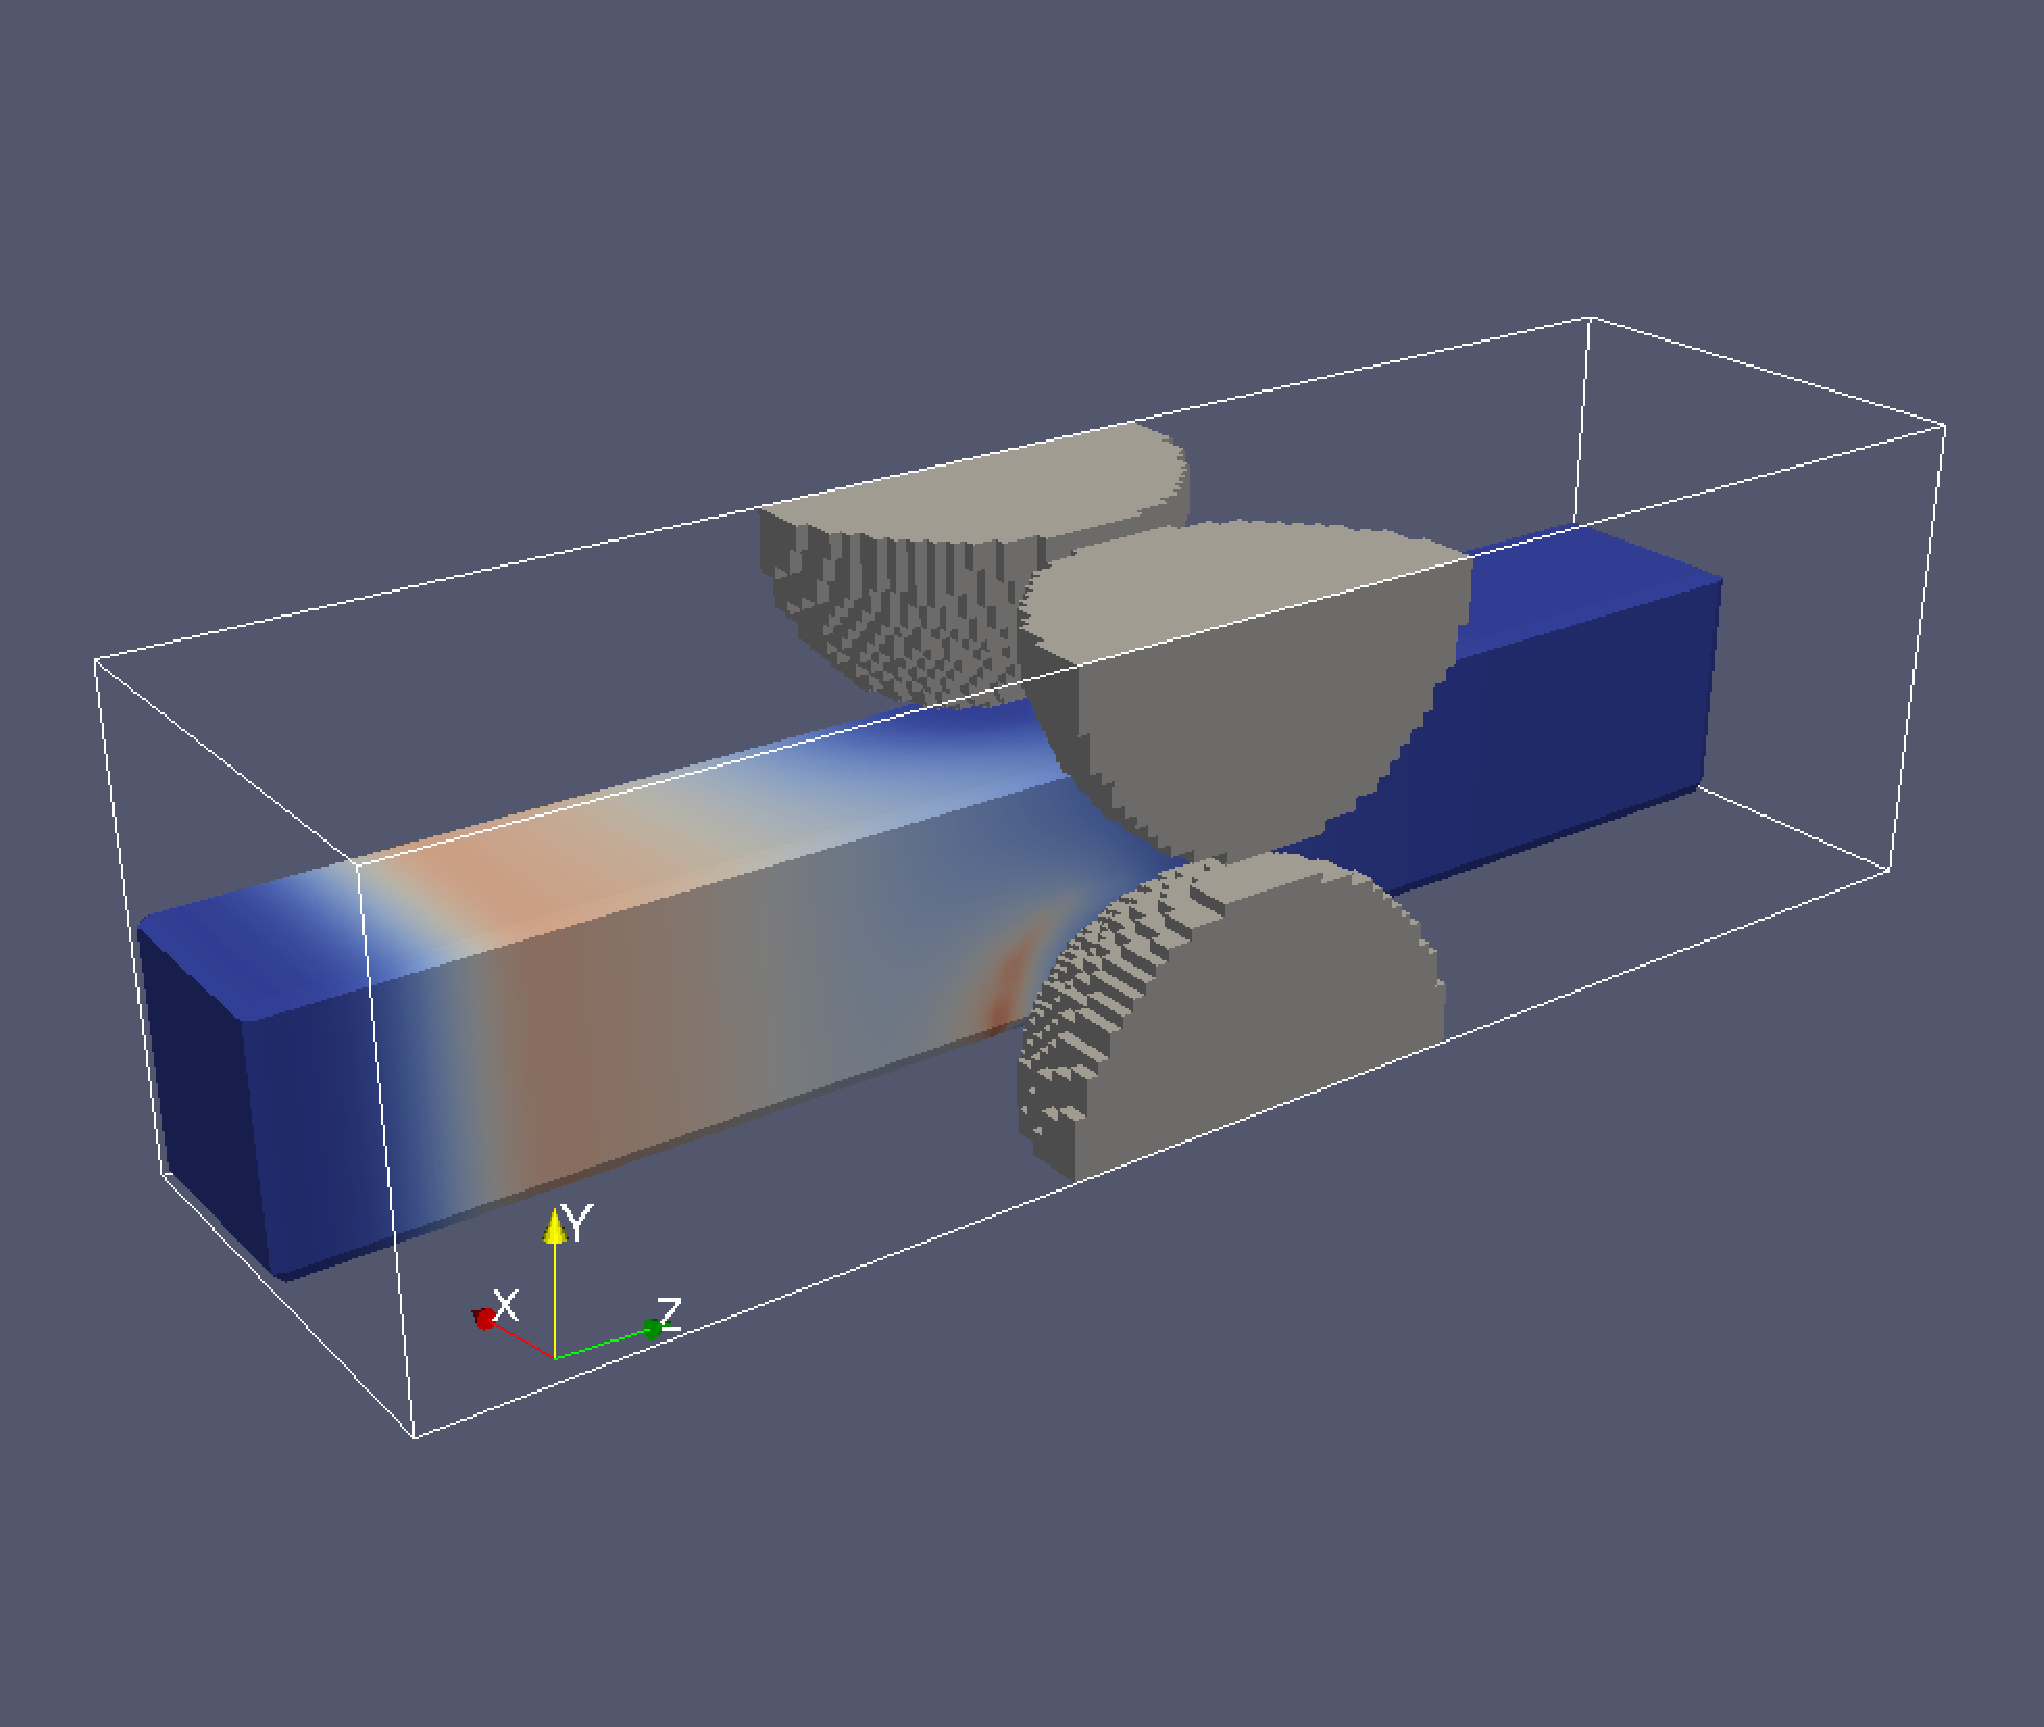
\includegraphics[width=10cm]{img/sim_screen.pdf} \label{fg_fdtdscreen} \end{figure} 
%}}}
\paragraph{Avoiding the near-field response in monitor planes} %{{{
\label{par_nearfield}
%% Hynek's trick
With the obvious exception of an effectively one-dimensional structure of layers perpendicular to the wave propagation, any other structure will change the orientation of the electric and magnetic fields. Such a perturbation of the field will be localized around the structure, and exponentially decaying with the distance in the form of an \textit{evanescent wave}.

An evanescent wave does not transport energy out of the structure into free space. However, some energy is stored in it. As a result, the energy can be transmitted to another structure if it approaches the zone of the evanescent wave, or, even if no energy is propagating by this means, the electromagnetic behaviour of a structure generally can be altered by its surroundings. Commonly this manifests itself e.g. as resonances shifting up or down in frequency.

The impact of the near-field reaching out of a structure to the s-parameters method is twofold:
\begin{enumerate}
 \item{First, computing a single layer of a metamaterial obviously more or less changes its behaviour. In the ideal case, a cell is surrounded by an infinite, periodic 3-D lattice of uniform cells.  Instead, in the s-parameter method, % FK: nebyly zavedeny?
the near-field spreads into free vacuum at the front and rear sides. 

This issue seems to be inherent to the method, but its impact can be assessed by simulating more than one unit cell. Generally, the retrieved $\Neff$ and $\Zeff$ values will change slightly with the number of layers being simulated: a single-cell simulation suffers the most from the absence of adjacent layers, whereas in a two-cell simulation the effect should be halved. Simulations of three (or more) cells result in a different behaviour of the cells at the surface and inside, which possibly broadens the resonance frequency and can supply intermediate results unsuitable to the retrieval method.
 } 
 \item{Second, the monitor planes can not distinguish between the evanescent or radiated waves, but only the latter are desired for the s-parameter computations. At very low frequencies or at frequencies around resonances, the near-field can significantly distort the retrieved parameters.

This can be resolved by adding \textit{padding} between the metamaterial cell and the monitor plane. As the evanescent field decays exponentially, usually a padding of less than half of the unit cell size is sufficient to suppress all artifacts due to near-field components. In contrast, the propagating waves only gain an additional phase offset that can be easily compensated after the simulation. } 
 \end{enumerate}
To the knowledge of the author, such a shift of monitor planes has not been employed in any related paper. It efficiently resolves the second issue, and it does so at an acceptable expense of moderately extending the simulation volume.
% TODO figure here a-b-c of different padding near a dielectric rod
%}}}
\paragraph{Scattering-parameter retrieval procedure} %{{{
The averaged electric and magnetic field recorded at the first monitor plane will be denoted as $E_{x}^{(1)}(t), H_{y}^{(1)}(t)$. Likewise, those at the second monitor plane will be denoted as $E_{x}^{(2)}(t), H_{y}^{(2)}(t)$. The amplitudes of typical time records are shown in a logarithmic scale in Fig. \ref{fg_sparam_timedomain}. 

The excitation pulse ca. 2 ps long excited in the structure two distinct resonances that both decayed exponentially in time with different decay rate, as is outlined by thin line segments. About 35 ps after the source was switched off, the stronger resonance reduces its intensity below that of the higher quality resonance, which can be clearly seen as a change of the decaying amplitude slope. The simulation time  was $t_{sim} =$ 150 ps.
\begin{figure}[ht] \centering \caption{Time-domain records of the fields in the s-parameter-based retrieval method; absolute values of the (complex) fields} 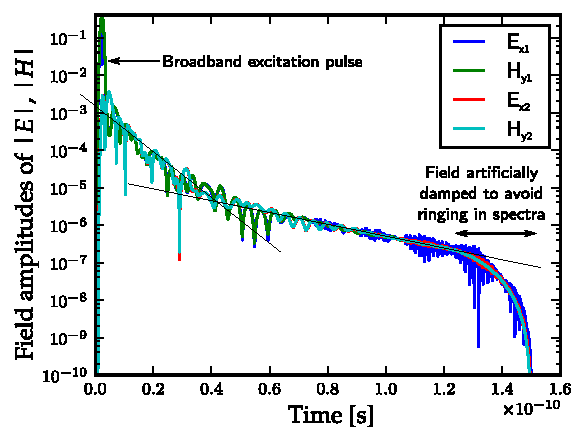
\includegraphics[width=9.5cm]{img/sim_timedomain_debug.pdf} \label{fg_sparam_timedomain} \end{figure}

%% Skutečný optimismus není věřit, že bude dobře, ale že budu mít v~každé situaci možnost, sílu a odhodlání učinit všechno k~tomu, aby lépe bylo. 

The spectral resolution is determined by the length of the time record. As a general rule, the higher quality of resonance, the sharper its spectral features. The case of a short time record significantly clipping a resonance ringdown is equivalent to coarse sampling on the frequency axis, which can not fully resolve the shape of the resonance. From the Fourier-Plancherel theorem %% TODO ref
it follows that the energy part stored in the clipped resonance will disappear from the frequency domain, too. As a result, characteristic ringing in the spectra will occur. Using the convolution theorem (see Sect. \ref{subsection_local_resp}), it can be deduced that applying a rectangular window in time domain results in a convolution with the sinc function in the spectrum. 

Using a time window that has smooth shape does not improve spectral resolution, but, in general, it suppresses the visually distracting ringing. Before further processing, all four time records were multiplied by the envelope function $g(t)$:
\begin{equation} 
\begin{split}
	g(t) 	& = 1 \text{ for } t < 0.8 t_{sim} \\
	g(t)    & = \frac{1 + \cos\left(\pi \frac{t/t_{sim}-0.8}{1-0.8}\right)}{2}  \text{ for } t > 0.8 t_{sim},
\end{split}
\label{eq_envelope}\end{equation}
which ensured that after 80 \% of the overall simulation time $t_{sim}$ the field starts dropping smoothly to zero, similar to the \textit{Hann window} function often used in digital signal processing. % TODO REF Hann window

By means of the Fourier transform, the fields can be converted to the frequency domain, which is simply denoted as $E_{x}^{(1)}(t) \rightarrow E_{x}^{(1)}(f)$, and so on. The results are shown in Fig. \ref{fg_sparam_timedomain}. 
\begin{figure}[ht] \caption{An illustration of how the electric field $\E$ (blue), magnetic field $\HH$ (light brown) and wave vector $\kk$ (thick arrow) are oriented in the waves registered in the simulation.}  \centering 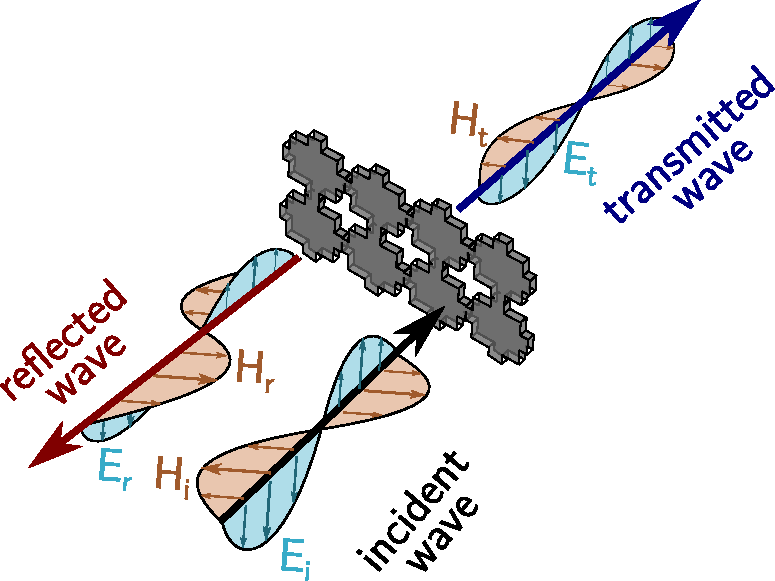
\includegraphics[width=8cm]{img/sim_separating_wave.pdf} \label{fg_separating_wave}\end{figure}

The monitor planes are assumed to be located in vacuum, and at a sufficient distance to eliminate the evanescent waves of the structure simulated. It follows that the vectors of the electric field $\E$, magnetic field $\HH$ and wave vector $\kk$ must a form right-handed triplet. %% TODO reference the M. E. solution
At both monitor planes, the forward and backward wave are linearly superposed as illustrated in Fig. \ref{fg_separating_wave}. Therefore they can be separated by the following relations: 
\begin{equation} 
	\begin{split}
		A^{(in 1)}(f)  := \frac{E_{x}^{(1)}(f) + Z_0 H_{y}^{(1)}(f)}{2}, \quad \quad \quad & A^{(out 1)}(f) := \frac{E_{x}^{(1)}(f) - Z_0 H_{y}^{(1)}(f)}{2}\\
		A^{(out 2)}(f) := \frac{E_{x}^{(2)}(f) + Z_0 H_{y}^{(2)}(f)}{2}, \quad \quad \quad & A^{(in 2)}(f)  := \frac{E_{x}^{(2)}(f) - Z_0 H_{y}^{(2)}(f)}{2}. 
	\end{split} 
\label{eq_separate_ampli}\end{equation}
The constant $Z_0$ stands for the \textit{vacuum impedance}, i.e. ratio of the electric and magnetic field of a freely propagating wave. Its physical value is $Z_0 = \sqrt{\mu_0/\varepsilon_0} = 4\pi c \cdot 10^{-7} \approx 376.7$ $\Upomega$ (but in the actual FDTD simulations, the built-in convention of $Z_0 = 1$ was maintained).

The wave separation result is plotted in Fig. \ref{fg_ampli}, and it allows a rough verification of the computation validity: the incident wave $A^{(in 1)}(f)$ should have smooth spectrum, as it is directly generated by the broadband source. The reflected wave $A^{(out 1)}(f)$ and the transmitted one $A^{(out 2)}(f)$ should be somewhat complementary to each other, with squares of their amplitudes summing up to the square of the incident wave (or less in case of losses). The fourth wave $A^{(in 2)}(f)$ should be negligible, as almost all wave energy is expected to be absorbed by the perfectly matched layers at the $z$-faces of the simulation volume. In practice it is nonzero, also due to numerical imprecision and remaining near-field components of the structure. In Fig. \ref{fg_separating_wave}, this relative error in amplitude is less than $10^{-3}$.
\begin{figure}[ht] \caption{Separated amplitudes of the forward and backward waves at the first and second monitor planes}  \centering 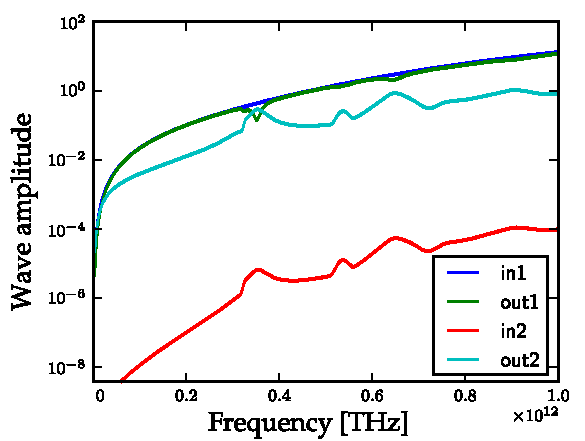
\includegraphics[width=10cm]{img/sim_ampli_debug_band.pdf}\label{fg_ampli} \end{figure} 

Finally, one can easily compute the complex scattering parameters $r(f)$ and $t(f)$ as the ratios of the reflected and transmitted wave amplitudes to the incident wave, respectively:
\begin{equation} 
	\begin{split}
		s_{11}(f) \equiv r(f) := \frac{A^{(out 1)}(f)}{A^{(in 1)}(f)},\\
		s_{12}(f) \equiv t(f) := \frac{A^{(out 2)}(f)}{A^{(in 1)}(f)}.
	\end{split}
\label{eq_sparam}\end{equation}
%}}}
\paragraph{Experimental verification of reflection and transmission} %{{{
\begin{figure} 
\caption{\textbf{a)} Electron microphotograph of the STO array (from \cite{nemec2009tunable}), 
\textbf{b)} dimensions of one unit cell thereof, with the orientation of the $\E$, $\HH$ and $\kk$ vectors}  \centering 
\textbf{a)} \mbox{\vspace{3cm} 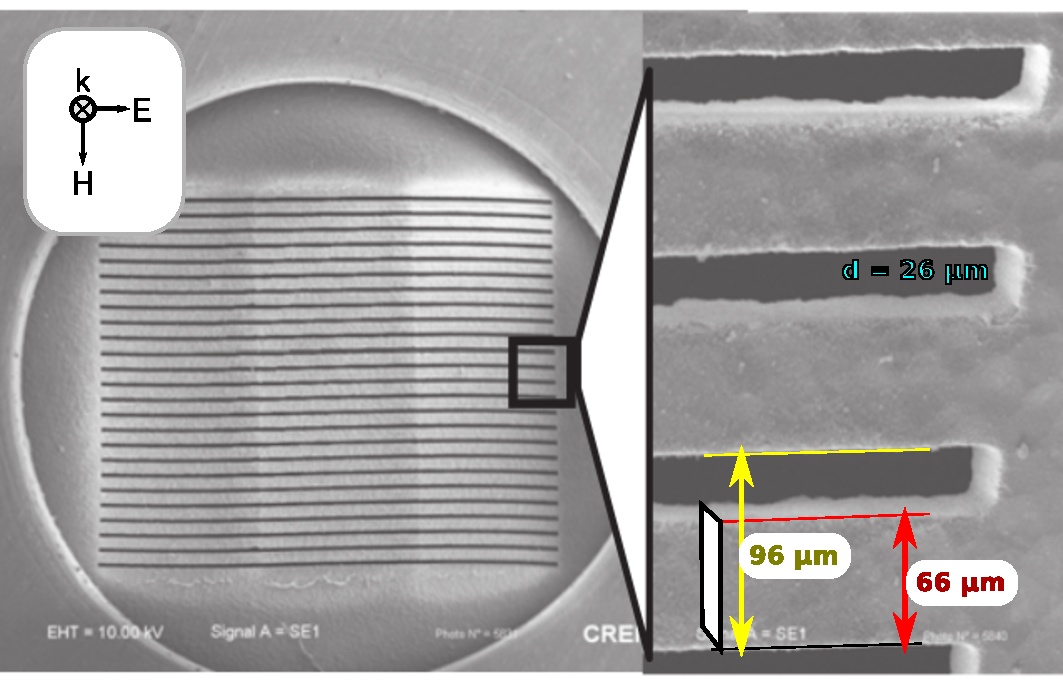
\includegraphics[width=9cm]{img/STOBar_photo.pdf}}  % 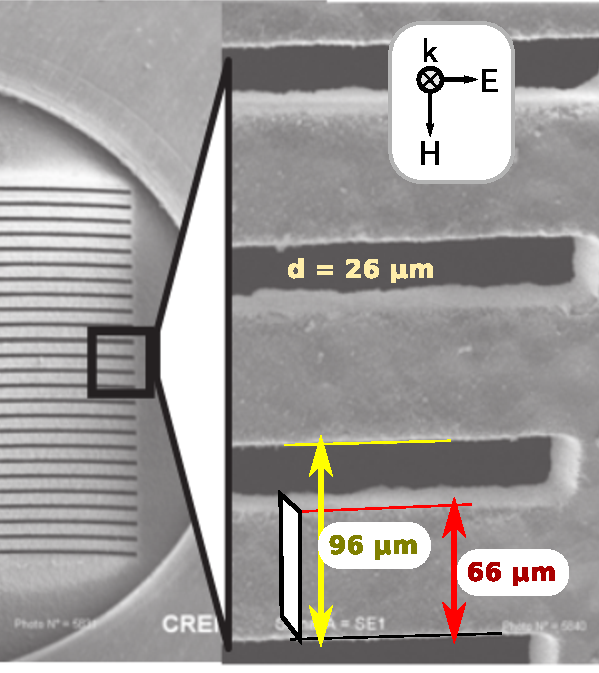
\includegraphics[width=5cm]{img/STOBar_photo_narrow.pdf}
\mbox{\textbf{b)} \mbox{\vspace{3cm}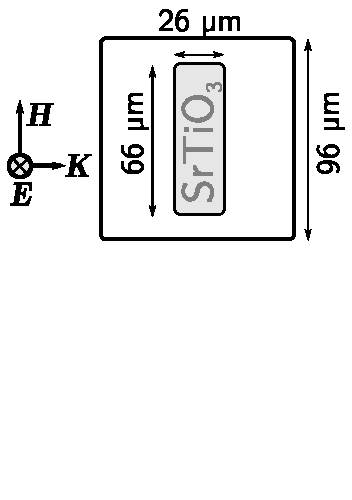
\includegraphics[width=5cm]{img/EBars_STO_sketch.pdf}} }
\label{fg_STO_bar_geom} \end{figure} 
To verify the simulation results against experimental data, we computed $r(f)$ and $t(f)$ for a structure that was measured previously in our terahertz laboratory.
It consisted of an array of high-permittivity dielectric bars, cut using a femtosecond laser % todo{what was the laser power and other parameters?
from a 26 $\upmu$m thick strontium titanate (STO) slab \cite{nemec2009tunable}. The periodicity was 96 $\upmu$m and the laser cut width was 30 $\upmu$m, resulting in 66 $\upmu$m width of each rectangular bar as shown in Fig. \ref{fg_STO_bar_geom}a,b. The permittivity of STO strongly depends on the temperature, and was not known a priori, so it was chosen as $\varepsilon_r(1\text{ THz}) = 365 + 62\ii$ for the simulation to match the experimental spectra.
\begin{figure} \caption{Experimental transmission $t_{exp}(f)$, compared to numerical reflection $r(f)$ and transmission $t(f)$ for strontium titanate bars $||\mathbf E$ of rectangular cross-section $26 \times 66\;\upmu$m. }  \centering 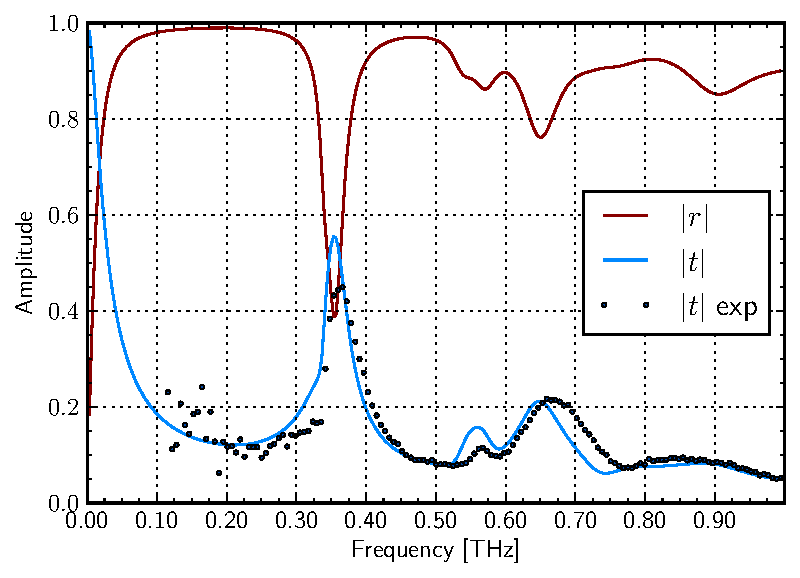
\includegraphics[width=12cm]{img/STObar_rt.pdf} \label{fg_STO_bar_rt} \end{figure} 
The curves computed using the FDTD simulations are compared to the experimental ones in Fig. \ref{fg_STO_bar_rt}, with a very good match in three well-resolved resonance peaks, and also in the high reflectivity ($|r| > 0.9$) in most of the spectrum which is caused by a great impedance mismatch between the dielectric and the surrounding air.

\begin{figure}[ht] \centering \caption{Parametric scan through the strontium titanate bar width, loss spectra computed as $1-|r^2|-|t^2|$. The bar width of 66 $\upmu$m is denoted by thin white line. Different modes are joined by black curves and their electric field shapes are drawn above the plot.} 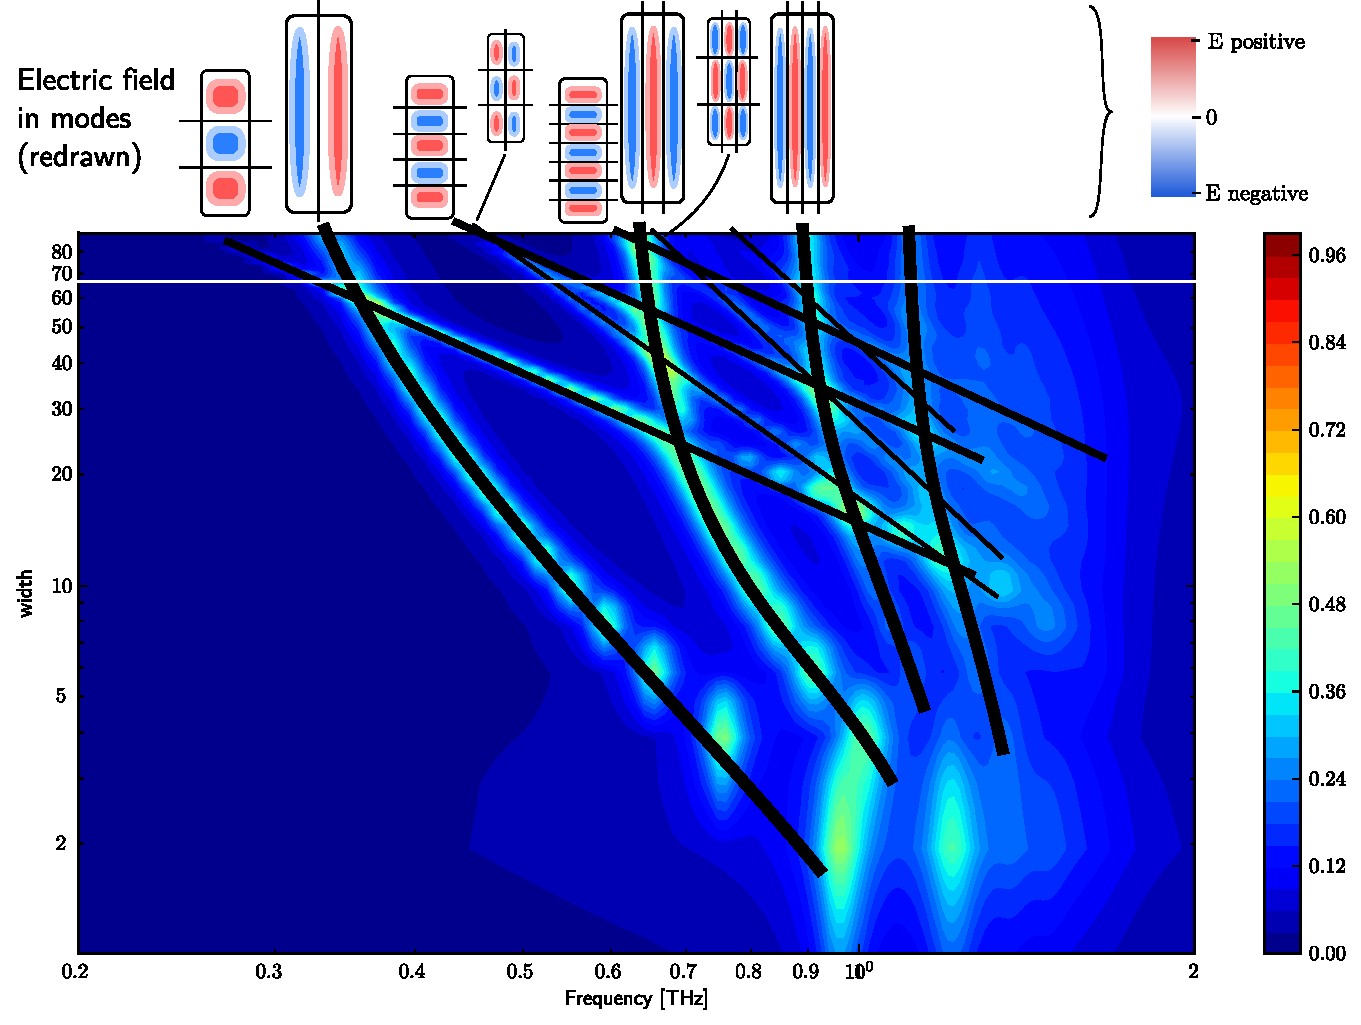
\includegraphics[width=\textwidth]{img/STOBarC_modes2.pdf} \label{fg_STO_bar_modes} \end{figure}
To briefly illustrate further possibilities of the numerical simulations, we scanned the relative width of the STO bar, and computed the relative energetic loss in the structure as $1-|r^2|-|t^2|$. Each loss peak can be clearly associated with one resonant mode in the dielectric, as shown in Fig. \ref{fg_STO_bar_modes}. The two-dimensional scan can reveal rich information about the underlying physics, most importantly, we see that the frequency at which different modes resonate has a different power dependence on the bar width. Note that both vertical and horizontal axes are logarithmic, so this exponent can be directly estimated from the slope of the line. Only modes with a mirror symmetry in the transverse direction ($y$-axis) couple to the wave.

It can also be seen from Fig. \ref{fg_STO_bar_modes} that around the bar width of 66 $\upmu$m, as denoted by the horizontal white line, there is actually a frequency cross-over of two modes, a narrow transverse one and a broader longitudinal one. This explains why in Fig. \ref{fg_STO_bar_rt} the first resonance has an obviously asymmetric shape in the simulated and experimental spectra.  %% This would form a typical Fano resonance if the losses were lower.
A more elaborate discussion of periodic structures composed of dielectric bars/rods oriented either along the electric or thee magnetic field will follow in the Sections \ref{sect_diel_rods_mag} and \ref{sect_diel_rods_el}.
%}}}
\paragraph{Retrieval of effective parameters} %{{{
So far, we computed the amplitude and phase of frequency-dependent reflectance $r(f)$ and transmittance $t(f)$ for a finite number of metameterial cell layers. 
These data, if supplied with the cell thickness $d$, are under some circumstances also sufficient to deduce the behaviour of a periodic structure composed of an infinity of such unit cells, i.e., to retrieve the effective parameters of the structure. 
\todo{this needs some discussion, if it is possible etc. ... or at least to get isofrequency contours if effparam do not exist, or if the method is too approximate}
To this end, we employ the Fresnel inversion and a custom way of obtaining physically meaningful  solution.
% TODO develop this somehow, cite Rockstuhs2004, relate to spatial dispersion and nonlocality - the evanescent field can be decomposed into dipoles, quadrupoles etc}
%It shall be noted that although the structure consists of a single layer, transmission and reflection is measured in the form of radiated waves to compute effective parameters for an infinite structure. The energy transferred by near field (evanescent wave) is neglected here. 
%The field components at the first monitor plane ($E_x^{(1)}, H_y^{(1)}$) and at the second one ($H_y^{(2)}, E_x^{(2)}$) give sufficient information for this, for instance at which frequencies are the photonic bands and which $K$-vector the wave will have. 

% todo check if symbols known
\textit{Fresnel coefficients} $r_1$, $t_1$ give the reflectance and transmittance from an interface of two homogeneous media described by their impedances $Z_1, Z_2$:
\begin{equation} r_1 = \frac{Z_2 - Z_1}{Z_2 + Z_1}, \quad \quad \quad t_1 = \frac{2 Z_2}{Z_2 + Z_1}, \quad \text{for perpendicular incidence}. \label{eq_fresnel}\end{equation}
Note that in the literature, the Fresnel coefficients are often expressed in a slightly different form, using the index of refraction $N$ instead of wave impedance $Z$; this holds only for common nonmagnetic media where $\mu_r = 1$ and therefore 
$$N \equiv \sqrt{\varepsilon_r \mu_r} = \sqrt{\mu_r/\varepsilon_r } \equiv 1/Z.$$ 
The complex reflectance $r_{s}$ and transmittance $t_{s}$ of a homogeneous slab with given wave impedance $z$, index of refraction $n$ and thickness $d$ can be computed by summing the infinite series of internal reflections.

\todo{add infinite sums for Fabry-Pérot resonances in a slab; develop expressions from Fresnel to effparam, and put into appendix?}
Knowing the complex $r(f)$ and $t(f)$ along with the sample thickness $d$, we may use the
classical algorithm \cite{smith2002determination}\cite[pp. 51-55]{shalaev2010book} to retrieve the effective index of refraction:
\begin{equation}
	N_{\rm eff} = \frac{\pm \arccos\left(\frac{1 - r^2+t^2}{2 t}\right) + 2\pi \cdot m}{k d},
\end{equation}
and the effective impedance:
\begin{equation}
	Z_{\rm eff}~= \pm \sqrt{\frac{(1+r)^2 - t^2}{(1-r)^2 - t^2}} \label{eq_Z}
\end{equation}
where $k = 2\pi f/c$ is the wave vector in vacuum and $c$ is the speed of light.

%}}}
\paragraph{Unambiguous arccosine} %{{{
The well-known complication of the described approach is that the arccosine and square root are ambiguous functions \cite{simovski2009material}. %% TODO change this cite?
%, yielding multiple solutions with different branches (indexed by an integer $m$) and signs. 
The sign and branch of the refraction index (indexed by an integer $m$), and the sign of wave impedance are not known a priori.  These three discrete-valued functions have to be selected during computation. The absence of discontinuities % TODO but they ARE discontinuities at low-loss resonances - rewrite this?
in the allowed photonic bands, passivity requirements % (Im$(N) \geq 0$, Re$(Z) \geq 0$) %% TODO FIXME check for the e+iomegat sign convention
and the Kramers-Kronig relations are a good verification of a correct solution. We have written routines that perform this task automatically after each FDTD simulation is run. Not knowing the correct branch of the index of refraction is equivalent to using the folded dispersion curves (cf. Par. \ref{par_disp_curv_per}), %% TODO refer to the theory
so the postprocesing of FDTD data corresponds to unambiguous \textit{unfolding} of the dispersion curves.

%See ~/p/MEEP_2013/130711_EWires/19_TiO2_cellscan_thick_HR/
\begin{figure} \centering \caption{\textbf{(a)} Real and \textbf{(b)} imaginary parts of the arccosine of complex argument $\upsilon$. Branch cuts are denoted with thick lines. The thick curve shows a possible trajectory of  $\upsilon(f)$ (upon a frequency variation), which intersects the branch cuts in points marked as R, L.\\ \textbf{(c)} From top to bottom: example function  $\upsilon(f)$, its ordinary arccosine, example branch and sign choices ensuring the continuity of the arccosine function, and the continuous version of $\arccos_{\mathrm{c}}(\upsilon)$, as determined by the algorithm described.} 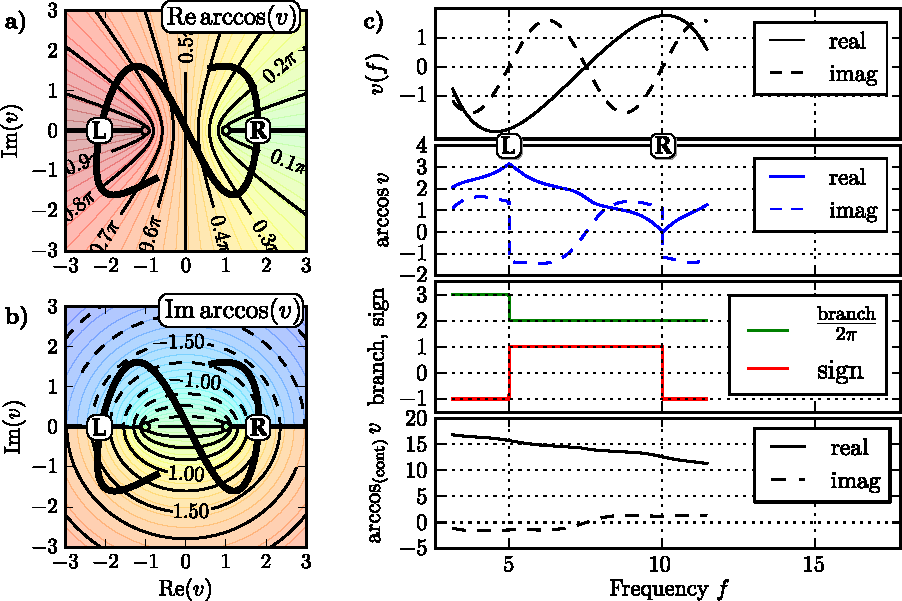
\includegraphics[width=16cm]{img/continuous_arccos/continuous_arccos_new.pdf} \label{fg_arccos}
\end{figure}
We deal with a passive medium, consequently we impose Im$(\Neff)>0$ %TODO WRONG, sign must be opposite
 and Re$(\Zeff)>0$. 
To facilitate processing of the results, we adopted an approach different from earlier published works \cite{smith2002determination,chen2004robust}
that ensures the continuity of effective parameters as a function of frequency on pure mathematical basis. This continuity, and the correct branch of the optical constants  %% TODO what missing?
can be ensured by choosing the branch conforming with
Kramers-Kronig relations if nonzero (but otherwise arbitrarily small) losses are introduced to the system. 
The important point consists in identifying the branch cuts of arccosine in the complex plane (Fig.\ \ref{fg_arccos}a,b). 
\begin{enumerate}
\item{
If, by increasing the frequency, the arccos argument, $v = (1 - r^2+t^2)/(2 t)$, passes through the right branch cut [i.e.  for $v= u+i 0$ where $u>1$], the real part of arccos$(v)$ touches zero, whereas the imaginary part is non-zero and changes its sign. The continuity is achieved if, from this frequency on, one reverses the sign of the arccos term (point "R" in Fig. \ref{fg_arccos}c). 
} 
\item{
The situation is slightly more complicated at the left branch cut [i.e. for $v = u+i 0$ with $u<-1$], where the imaginary part of $\arccos(v)$ experiences again a step-like change of the sign and the real part reaches the value of $\pi$. The continuity is then restored upon a sign reversal accompanied by a branch index change,  illustrated by the point "L" in Fig. \ref{fg_arccos}c. 
} 
 \end{enumerate}
The correct reconstruction of the arccosine therefore only requires to compute the integer-valued branch along with the sign, both being functions of frequency. The sign of the square root function is again chosen such than $Z$ is a continuous function of frequency.  


%}}}
\paragraph{Applicability of the method}%{{{
\add{
this method makes several assumptions that may not always hold. One of them is that nearly all of energy is transferred by the radiated wave, in which case the metamaterial is sometimes described as a \textit{Bloch lattice} \cite{simovski2007bloch, andryieuski2012bloch}. In other cases, usually in dense and particularly in metallic structures, a significant amount of energy is transferred by the near-field coupling, and it can be demonstrated that the effective parameters retrieved by this method strongly depend on the number of layers \cite{rockstuhl2008transition,andryieuski2010homogenization} which renders the approach invalid.
}

% TODO add when the parameter $v$ passes too close to the ends of branch cuts ... 

%%% It is also known that the phase of the reflectance depends on the surface termination for noncontinuous materials. In the cases where the wavelength of the radiation in the material is much larger than the unit cell dimensions this ambiguity becomes small. A useful control of the effective sample properties can be made by changing the thickness of the sample (number of unit cells along the wave vector). We have chosen a symmetric geometry where the dielectric rod is positioned in the center of a square unit cell and the overall thickness of the sample is an integer multiple of the unit cell size. In this geometry the retrieved effective parameters of our structure depend only negligibly on the number of unit cells that we put in the $z$-direction.
%%% 
%%% \cite{menzel2008retrieving} s-param methdo extended under oblique incidence

% TODO add    A review of the scattering parameter extraction method with clarification of ambiguity issues in relation to metamaterial homogenization

%}}}
\paragraph{Summary of the scattering parameters retrieval method} %{{{
% TODO In many works cited here, the multiplicity of the branches is mentioned as a major obstacle, however we devised a 
% relatively simple and mathematically straightforward method to find the correct solution, that works reliably for 
% structures with nonzero losses.
% As a much more important issue we should mention this method can never exactly simulate the metamaterial cell in its infinitely periodic lattice, and that   %% as is discussed above.


% Numerous modifications of this method have been made \cite{Hasar2009, Arslanagic2012}
%}}}

\subsection{Current-driven homogenisation} % TODO
\begin{figure}[ht] \centering \caption{CDH \todo{+CAPT, MOVE, and add the X-Y-Z arrows to the figure}} 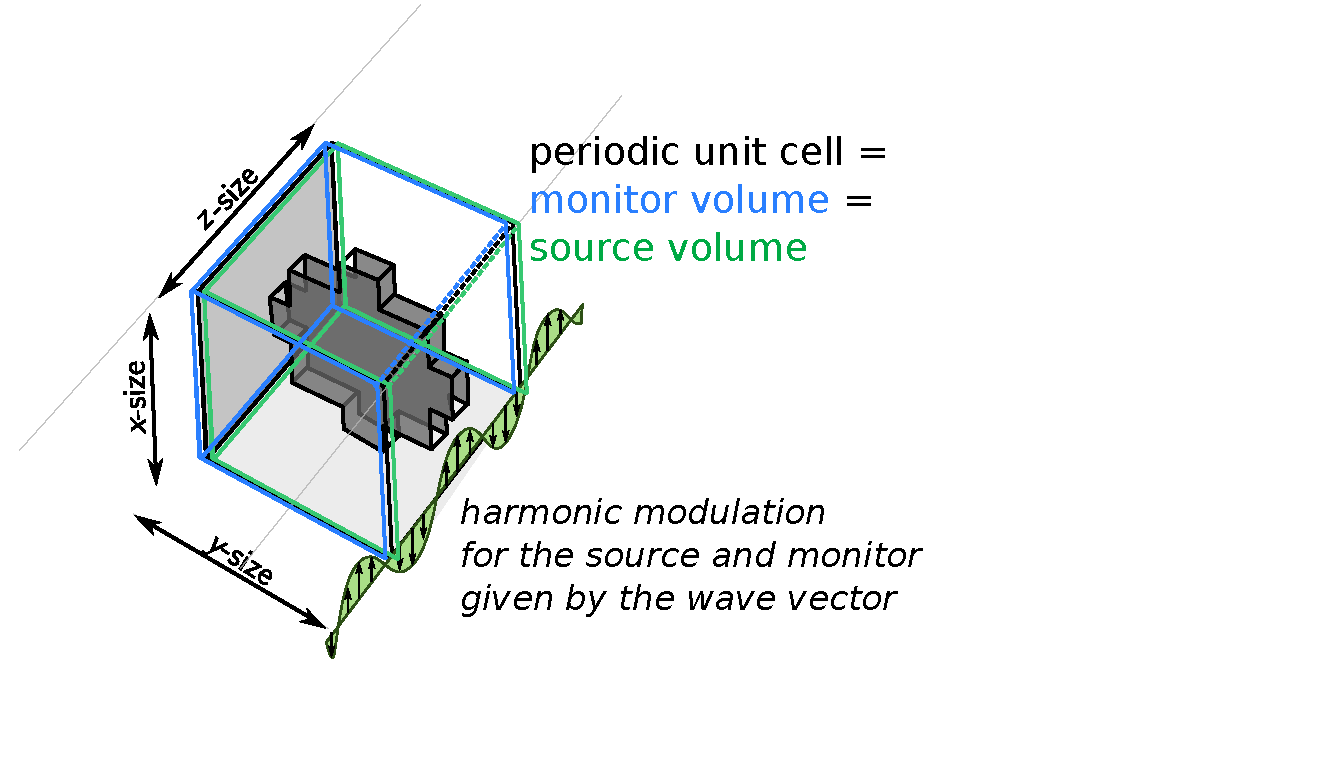
\includegraphics[width=12cm]{img/cdh_geometry.pdf}  \label{fg_fdtd_cdh} \end{figure} %% 
%% Markel2013: Of course, a refractive index per se (generally, tensorial and dependent on the direction of the Bloch wave vector) can always be formally intro- duced for a Bloch wave.

\add{
\paragraph{Simulation setup}
\paragraph{Retrieving the structure response}
\paragraph{Identification of dispersion curves}
\paragraph{Retrieval of effective permittivity out of dispersion curves}
\paragraph{Comparison with the scattering-parameters method}
}
%\begin{figure} \caption{img/cdh\_srrwire\_structure.pdf}  \centering 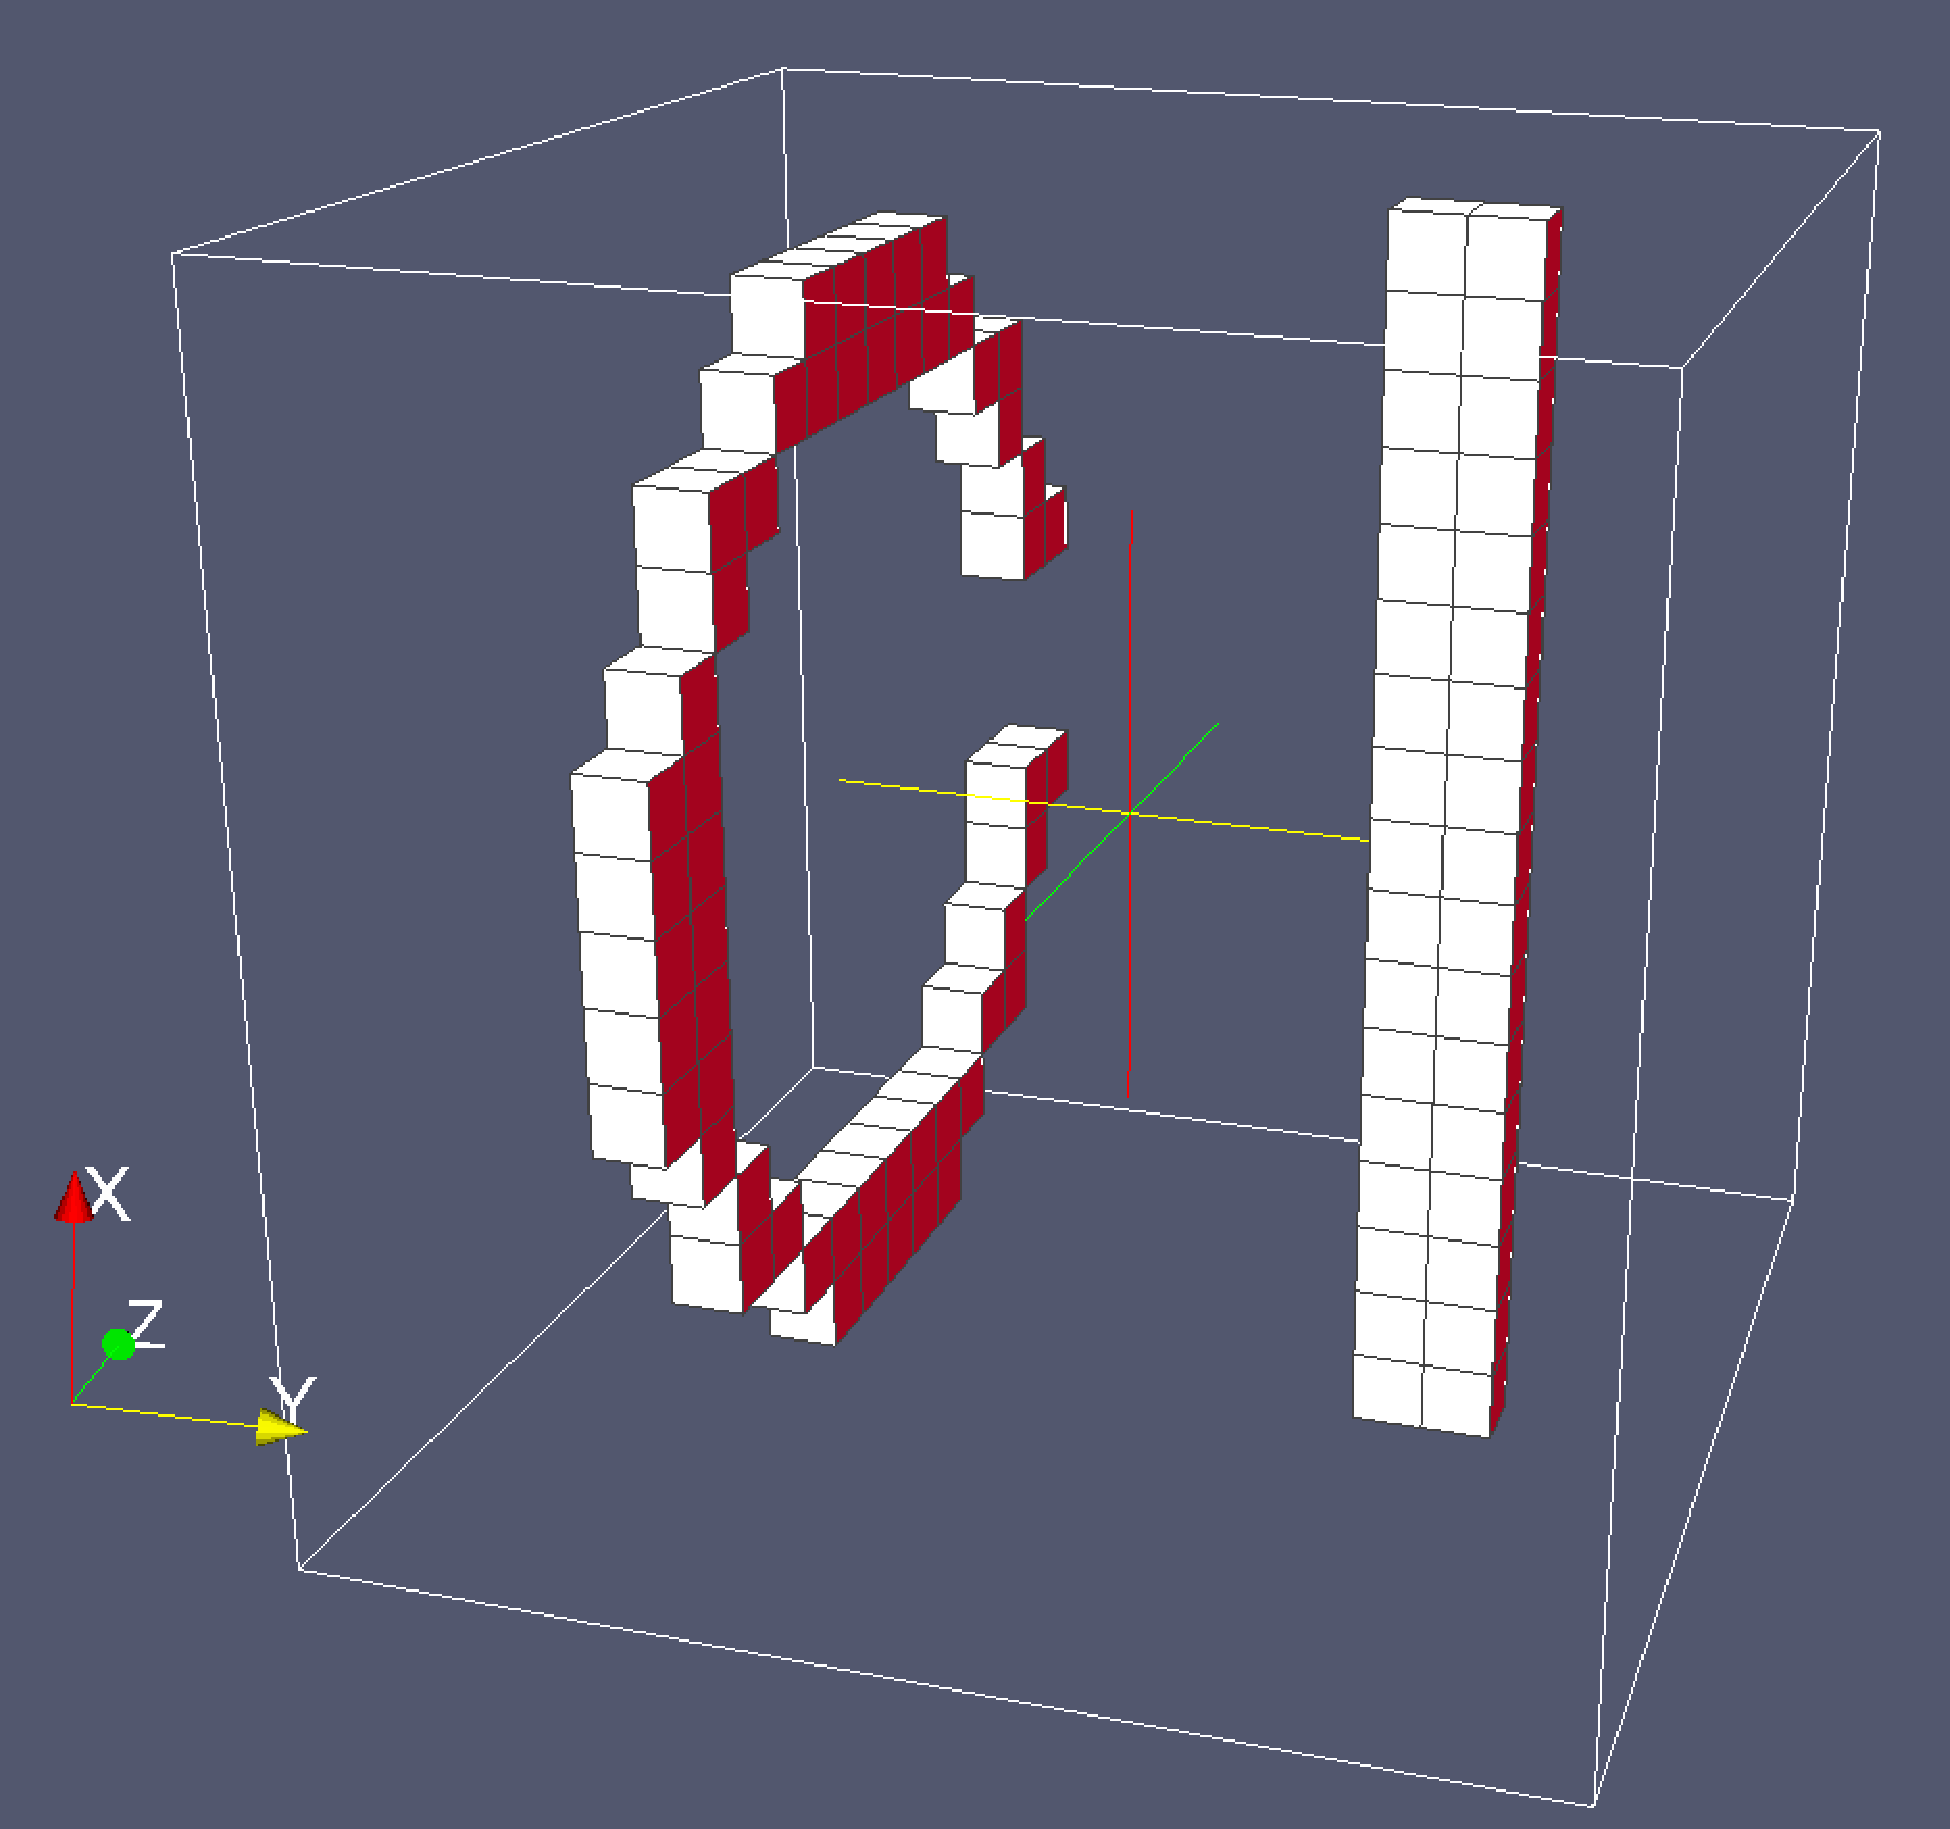
\includegraphics[width=8cm]{img/cdh_srrwire_structure.pdf} \end{figure} 
%\begin{figure} \caption{img/cdh\_srrwirethick.pdf}  \centering 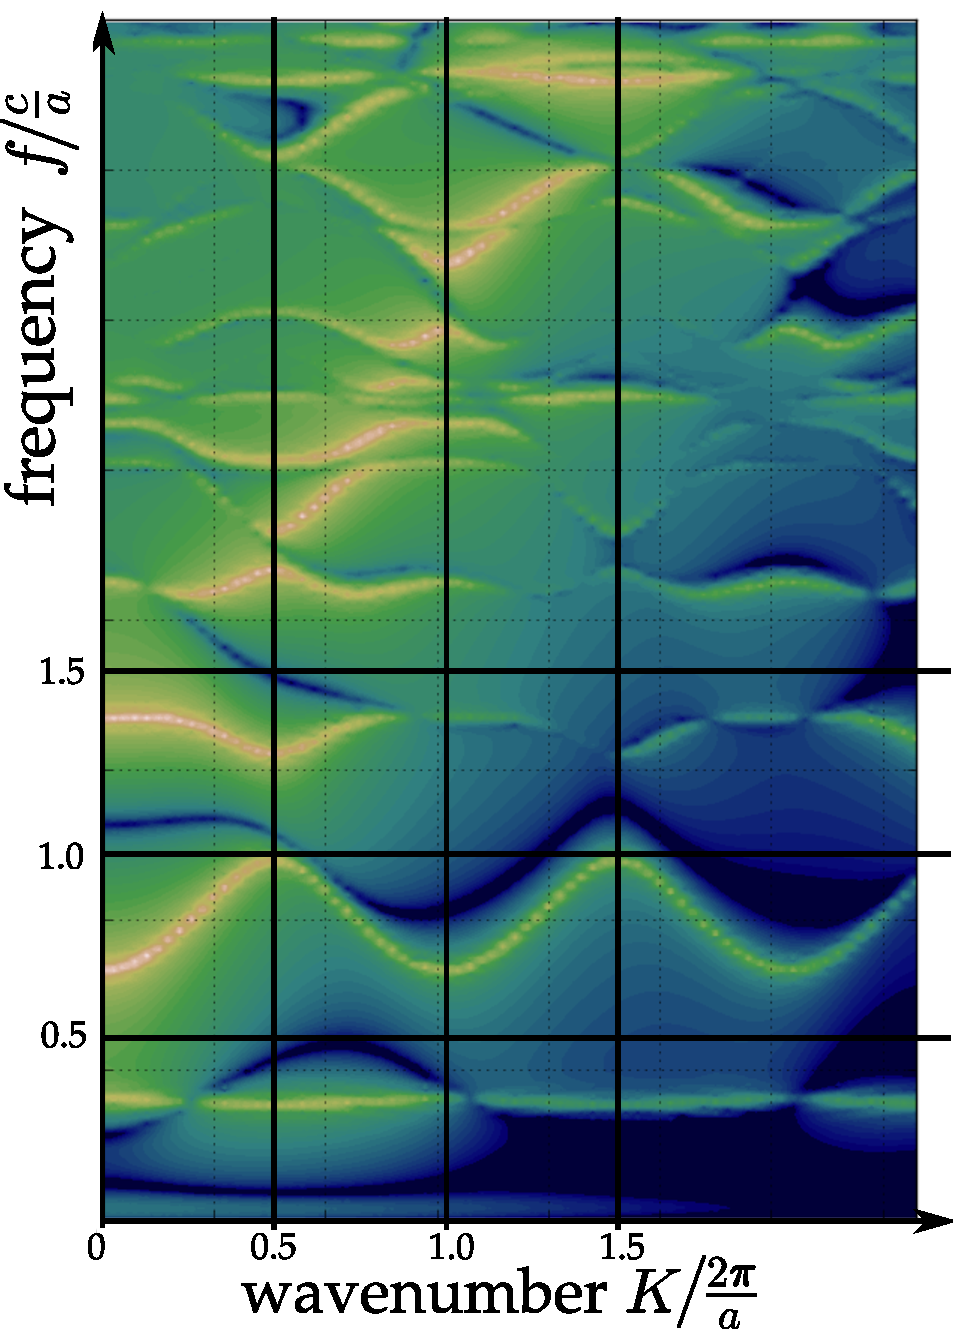
\includegraphics[width=6cm]{img/cdh_srrwirethick.pdf} \end{figure} 

%% \subsection{Simulation of refraction on a wedge} % ... shall I write this?
%% \mdf{
%% \paragraph{Simulation setup}
%% \paragraph{Derivation of the beam deflection angle}
%% \paragraph{Why the beam deflection angle depends on beam direction}
%% \paragraph{Analysis of spatio-temporal spectrum}
%% \paragraph{Limitations of this method}
%% }


\subsection{Other effective parameter retrieval methods} % TODO
\mdf{TODO
% TODO read: http://scholar.google.cz/scholar?q=Tsukerman+2011++of+metamaterial+Rigorous+Whithey+interpolation&btnG=&hl=cs&as_sdt=0%2C5

WPRM (Wave Propagation Retrieval Method), \cite{andryieuski2010homogenization}: review of restoration methods ("standard method, field averaging, quasimode theory, wave phenomena")

only reflection (single-interface) problem, \cite{yang2010retrieving} 

only transmission? \cite{hasar2009new} 
%%% /home/filip/PhD/Sources\_MM\_theory/120626\_Homogenisation\_approaches
}

